%% LyX 2.4.1 created this file.  For more info, see https://www.lyx.org/.
%% Do not edit unless you really know what you are doing.
\documentclass[english,american]{article}
\usepackage[T1]{fontenc}
\usepackage[utf8]{inputenc}
\usepackage{color}
\usepackage{babel}
\usepackage{float}
\usepackage{graphicx}
\usepackage{rotfloat}
\usepackage{setspace}
\usepackage[]
 {hyperref}

\makeatletter
%%%%%%%%%%%%%%%%%%%%%%%%%%%%%% User specified LaTeX commands.
%%base:
\usepackage{amsfonts}
\usepackage{setspace}
\usepackage{fullpage}
\usepackage{rotating}
\usepackage{booktabs}
\usepackage[abbr]{harvard}
\usepackage{color}

\renewcommand{\floatpagefraction}{.99}
\renewcommand{\topfraction}{.99}
\renewcommand{\bottomfraction}{.99}
\renewcommand{\textfraction}{0.01}

%%Cross reference figs and tabs
\AtBeginDocument{%
\let\ref\autoref
\renewcommand\figureautorefname{\@gobble}
\renewcommand\tableautorefname{\@gobble}
\renewcommand\equationautorefname{\@gobble}
}

\usepackage{color}
\hypersetup{colorlinks,linkcolor=blue}

\usepackage[toc,page]{appendix}



%%independence symbol
\newcommand\independent{\protect\mathpalette{\protect\independenT}{\perp}}
\def\independenT#1#2{\mathrel{\rlap{$#1#2$}\mkern2mu{#1#2}}}

%%or indep
\usepackage{graphicx}
\newcommand{\indep}{\rotatebox[origin=c]{90}{$\models$}}

%\usepackage[nolists,tablesfirst]{endfloat}
%\nomarkersintext

%\DeclareDelayedFloatFlavor{sidewaystable}{table}
%\DeclareDelayedFloatFlavor{sidewaysfigure}{figure}

\usepackage{graphicx,dblfloatfix}


% set hyperlink color
\usepackage{url}
\hypersetup{urlcolor=blue}

%%insert quote
\usepackage{epigraph}
\renewcommand{\textflush}{flushepinormal}
\setlength{\epigraphwidth}{0.9\textwidth}

% insert online Appendix: appendix page numbering
\let\origappendix\appendix % save the existing appendix command
\renewcommand\appendix{\clearpage\pagenumbering{roman}\origappendix}

% modify a page's margin e.g. abstract page
\usepackage{changepage}

%supress reference label/number

%change arabbic to roman numeral?
\renewcommand\thesection{\Roman{section}}
%\renewcommand\thesubsection{\Alph{subsection}}

%set some pages portrait?
\usepackage{pdflscape}


\usepackage[T1]{fontenc}

%stop table exceeding page
\usepackage{graphicx}

%include link in tex tables
\usepackage{url} 

%remove numbering of references
%\makeatletter
%\renewcommand\@biblabel[1]{}
%\makeatother

\usepackage{threeparttablex} % for footnote after longtable

\makeatother

\begin{document}
\selectlanguage{english}%
\thispagestyle{empty} \doublespace\begin{adjustwidth*}{+1.cm}{+1.cm}
\begin{center}
{\large\textbf{Appendix for }}{\large\par}
\par\end{center}

\begin{center}
{\large\textbf{THE VALUE OF COMMUNICATION FOR MENTAL HEALTH}}{\large\vspace*{0.5cm}
\hspace{1cm}Francis Annan$^{\clubsuit}$ \hspace{4cm}Belinda Archibong$^{\spadesuit}$}\\
{\small University of California, Berkeley and NBER\hspace{1cm}Johns
Hopkins University SAIS and NBER}{\large}\\
\textbf{ JULY 2025}
\par\end{center}

\end{adjustwidth*}\begin{adjustwidth*}{+1.1cm}{+1.1cm}{\large\vspace*{0.5cm}
}{\large\par}
\selectlanguage{american}%
\begin{center}
\par\end{center}

\selectlanguage{english}%
\setcounter{figure}{0} \renewcommand{\thefigure}{A\arabic{figure}}
\setcounter{table}{0} \renewcommand{\thetable}{A\arabic{table}}

\section{\textcolor{black}{Appendix}}

\subsection{Global Review of Communication Programs -- Motivating Evidence I}
\begin{center}
\begin{sidewaystable}
\caption{\textbf{A G}{\footnotesize\textbf{LOBAL REVIEW OF COVID-19 COMMUNICATION
INTERVENTIONS}}{\scriptsize\textbf{ }}}\label{fig:globalreviewp1}

\setlength{\pdfpagewidth}{8.5in} \setlength{\pdfpageheight}{11in}
\tiny
\begin{tabular}{lclcc}
\multicolumn{5}{c}{} \\ \hline  \hline
\textbf{Setting} & \textbf{Entity} & \textbf{Details and source(s)} & \textbf{Date started} & \textbf{Date ended} & \\ \hline

\textbf{United} & Government & *FCC launched the program Keep Americans Connected in which communications companies agreed on & 03/13/2020 & 06/30/2020 \\
 \textbf{States} & \textbf{FCC} & not terminating the internet services of Americans in case they do not keep up to date with payments of &  &  \\ 
  &  & internet and telephone bills in response to the COVID-19 crisis. The companies opened their Wi-fi hotspots &  &  \\ 
  &  & for the population. &  &  \\ 
  &  &  &  &  \\
  &  & *FCC also maintained other communication initiatives during the pandemic such as granting ATT to use & 03/26/2020 & 05/25/2020  \\ 
  &  & additional spectrum in Puerto Rico and Virgin Islands in order to improve and expand the internet &  &  \\ 
  &  & connectedness in these territories (60 days period).  &  &  \\ 
  &  &  &  &  \\
  &  & *FCC waived temporarily its rules to Inteliquent to Zoom and WebEx in order to stimulate and help & 03/27/2020 & 06/30/2020 \\ 
  &  & consumers who now need strictly in these services to study and work. & & \\ 
  &  & \textbf{Source:} \url{https://www.fcc.gov/keep-americans-connected}  &  &  \\ \hline
  & Companies &  \textbf{ATT Inc.:} *Provided free 10GB of internet data per month for 60 days as a temporary relief to eligible & 03/27/2020 & 05/26/2020 \\  
  &  & customers to be able to stay connected during the difficult times, starting March 27, 2020. &  &  \\ 
  &  & \textbf{Source:} \url{https://about.att.com/newsroom/2020/covid_19_att_prepaid.html}  &  &  \\ 
  &  &  &  &  \\
  &  &  \textbf{Comcast Corp.:} Provided essential internet and mobile services without charge to low-income families, & Not available  & Not available \\  
  &  & including seniors, veterans and people with disabilities in the United States. &  &  \\ 
  &  & \textbf{Source:}  \url{https://corporate.comcast.com/covid-19}  &  &  \\
  &  &  &  &  \\
  &  &  \textbf{Amazon:} *Donated 8,200 laptops to students who attend public schools in Seattle and 4,000 laptops for  & 04/06/2020 & -- \\ 
  &  & high school students across the US through the Amazon Future Engineer program. &  &  \\ 
  &  & *Made many videos on Amazon Prime free for anyone during the stay at home orders period. Content  &  03/04/2020 & Not available \\ 
  &  & included cartoons and family friendly movies. In addition to that, Amazon made many of its books free for &  &  \\ 
  &  & the public who could download them as PDFs. &  &  \\ 
  &  & \textbf{Source:} \url{https://www.aboutamazon.com/news/company-news/amazons-covid-19-blog-updates-on-how-were-responding-to-the-crisis} &  &  \\
  &  &  &  &  \\
  &  &  \textbf{Microsoft:} *Microsoft has supported the local education of Washington state during the Pandemic by making the  & 03/16/2020 & Not available  \\ 
  &  & Virtual Classroom and Teams available for free. It has also created training sessions for teachers of the &  &  \\ 
  &  & state and helped schools in the districts to increase their phone lines to accommodate more parents and &  &  \\ 
  &  & students’ phone calls. &  &  \\ 
  &  & *Microsoft is also working with the Washington state’s government to build more broadband spots around &  &  \\ 
  &  & the state to help more people have access to the internet through the Airban initiative. The company also &  &  \\ 
  &  & brought emergency coverage to 29 school districts of the state. &  &  \\ 
  &  & \textbf{Source:} \url{https://news.microsoft.com/on-the-issues/2020/04/17/microsoft-covid-19-washington-state/}  & &  \\ \hline
  
\textbf{Ghana} & Government & The Government reduced the Communication Service Tax (CST) from 9pct to 5pct which reflected a reduction & 09/15/2020 & Ongoing \\
  & & in the cost of mobile talk time and data purchases, effective September 15, 2020 in response to COVID-19 &  &  \\ 
  &  &  &  &  \\
  &  & \textbf{Source:} \url{https://gra.gov.gh/domestic-tax/tax-types/communication-service-tax/}  & &  \\ \hline

\textbf{Brazil} & Government & *The government signed an agreement with Cisco  in late May in order to launch the program “Brasil & 05/27/2020 & Ongoing \\
  & & Digital e Inclusivo” (Digital and Inclusive Brazil) that has as its goal to accelerate the technological and &  &  \\ 
  & & digital development of the country. As a response to the COVID-19 crisis, the program aims to facilitate &  &  \\ 
  & & and accelerate telemedicine in the country. &  &  \\ 
 &  &  &  &  \\
  & & *13.6 million of Brazilians live in the “favelas” (slums) and usually have restricted access to technology and & 03/DD/2020 & Ongoing \\ 
  & & communication systems. In this way, in order to bring awareness about the pandemic to the most &  &  \\ 
  & & vulnerable in Brazil, NGOs, journalists and activists have used alternative methods of communication in &  &  \\ 
  & & the population. &  &  \\
  &  &  &  &  \\ 
  & & *The Brazilian government launched a  program to distribute technological equipment and access to the & 09/18/2020 & Ongoing \\ 
  & & internet for students of the public school system in the country. The initiative will cost approximately  &  &  \\ 
  & & R$2.5 billions and the Brazilian Agency of Communications (Anatel) will be responsible to implement it and &  &  \\ 
  & & distribute the materials. &  &  \\ 
  &  & \textbf{Source:} \url{https://newsroom.cisco.com/feature-content?type=webcontent&articleId=2076852} & &  \\ \hline
 
\textbf{Ecuador} & Government & Similar to the most Favelas communities in Brazil, Ecuador also has a significant population that has  & 03/DD/2020 & Not available \\
  & & limited access to technology and communication channels. These are indigenous communities in which the  &  &  \\ 
  & & government and other organizations such as UNESCO have approached in regards to the pandemic in a  &  &  \\
  & & very strategic way. They have been taking advantage of the communication channels that the indigenous  &  &  \\ 
  & & communities have even though they are very scarce. Webpages directed to these communities that &  &  \\ 
  & & address COVID were created, audios and videos were produced by UNESCO and the organizations as well   &  &  \\ 
  & & as others have been conducting cultural activities with the communities in order to bring awareness and &  &  \\ 
  & & information about the pandemic. &  &  \\ 
 &  &  &  &  \\
  &  & \textbf{Source:} \url{https://en.unesco.org/news/media-and-communications-indigenous-peoples-pandemic}  & &  \\ \hline 
  
  \textbf{Global} & Company-& \textbf{#ZoomTogether} & 11/26/2020 & 11/27/2020 \\ 
  \textbf{/United States} & \textbf{Zoom} & Zoom removed the 40 minutes time limit for free accounts during Thanksgiving as an initiative to help &  &  \\
   & & families and friends communicate during the holiday season even if they were distant to each other &  &  \\
   & & During Thanksgiving Day, anyone was able to make video conferences longer than 40 minutes through &  &  \\
   & & Zoom without being interrupted. &  &  \\
  &  &  &  &  \\
  &  & \textbf{Source 1:} \url{https://www.cnn.com/2020/11/17/tech/zoom-time-limit-thanksgiving-trnd-wellness/index.html}  & &  \\ \hline \hline

\end{tabular}




\end{sidewaystable}
\par\end{center}

\begin{center}
\begin{sidewaystable}
\caption{\textbf{CONT'D: A G}{\footnotesize\textbf{LOBAL REVIEW OF COVID-19
COMMUNICATION INTERVENTIONS}}{\scriptsize\textbf{ }}}\label{fig:globalreviewp2}

\setlength{\pdfpagewidth}{8.5in} \setlength{\pdfpageheight}{11in}
\tiny
\begin{tabular}{lclcc}
\multicolumn{5}{c}{} \\ \hline  \hline
\textbf{Setting} & \textbf{Entity} & \textbf{Details and source(s)} & \textbf{Date started} & \textbf{Date ended} & \\ \hline

 \textbf{Global} & Company-& *Google has donated USD10 million for Distance Learning Fund that supports organizations across the  & 03/DD/2020 & -  \\ 
  & \textbf{Google} & globe which help students who have had to adapt to online learning but do not have access to resources to do so &  &  \\
  &  &  &  &  \\
  & & *Google has also partnered with many universities around the world and distributed AI tools and & 03/DD/2020  & Not available  \\ 
  & & mechanisms to help them keep track of the development of COVID-19 in the world and spread information &  &  \\ 
  & & about it for all. &  &  \\ 
   &  &  &  &  \\
  &  & \textbf{Source 1:} \url{https://www.google.org/covid-19/#distance-learning}  & &  \\ 
  &  & \textbf{Source 2:} \url{https://blog.google/outreach-initiatives/google-org/google-supports-covid-19-ai-and-data-analytics-projects/}  & &  \\ \hline

\textbf{Global} & Company-& *Transperfect  has been translating and delivering materials and information about COVID-19 across the & 04/DD/2020 & Not available \\ 
  & \textbf{Transperfect} & globe. The work has been so helpful that the company won the International Business Award for COVID-19 &  &  \\
  & & Communication Initiatives. &  &  \\ 
  &  &  &  &  \\
  & & *The company produced videos of COVID-19 prevention tips in more than 11 languages and personalized &  &  \\ 
  & & it for companies for free. &  &  \\ 
 &  &  &  &  \\
  &  & \textbf{Source:} \url{https://www.prnewswire.com/news-releases/transperfect-wins-international-business-award-for-covid-19-communications-initiatives-301134747.html}  & &  \\ \hline 
  
 \textbf{Europe and } & Companies-& These companies have been slowing down and decreasing the streaming quality of their videos since   & 04/01/2020 & 04/30/2020 \\ 
 \textbf{United States} & \textbf{Netflix,} & March in Europe and also in the US. The initiative is an attempt to help with the internet traffic and higher &  &  \\
   & \textbf{Youtube,} & latency and packet loss caused by the high usage of the internet by households after stay at home orders &  &  \\
   & \textbf{Streaming services} & took place in Europe and in the US (30 days period). &  &  \\
   &  &  &  &  \\
   &  & \textbf{Source 1:} \url{https://www.cnn.com/2020/03/19/tech/netflix-internet-overload-eu/index.html}  & &  \\ 
  &  & \textbf{Source 2:} \url{https://latest-news-viral.blogspot.com/2020/03/streaming-in-time-of-covid-19-youtube.html}  & &  \\  \hline
 
\textbf{Global} & Company-& *Facebook has been partnering with governments in order to spread accurate information about the & 03/DD/2020 & Not available \\ 
  \textbf{/India} & \textbf{Facebook} & pandemic. An interesting and important partnership was with India’s government that has been relying a &  &  \\
   & & lot on social media in order to spread awareness and information about COVID-19. Other than social &  &  \\
   & & media, Indian local governments have also developed and used apps that monitor COVID-19 in the &  &  \\
   & & country, by using Information and Communications Technology (ICT) and Artificial Intelligence (AI). &  &  \\
   & & &  &  \\ 
  & & *These apps are helpful and very informative, but a significant part of the population in India does not &  &  \\ 
  & & have access to the internet which shows how the Digital Divide in India has deepened the social, health &  &  \\ 
  & & and educational inequalities in the country. &  &  \\ 
  &  &  &  &  \\
  &  & \textbf{Source 1:} \url{https://about.fb.com/news/2020/11/coronavirus/;}  & &  \\ 
  &  & \textbf{Source 2:} \url{https://www.bbc.com/news/world-asia-india-53471749}  & &  \\ 
  &  & \textbf{Source 3:} \url{https://www.weforum.org/agenda/2020/10/how-covid-19-deepens-the-digital-education-divide-in-india/}  & &  \\ 
  &  & \textbf{Source 4:} \url{https://academiccommons.columbia.edu/doi/10.7916/d8-bbw6-yt70}  & &  \\ 
  &  & \textit{Download the paper to see all the apps created} & &  \\ 
  &  & \textbf{Source 5:} \url{https://www.weforum.org/agenda/2020/10/how-covid-19-deepens-the-digital-education-divide-in-india/}  & &  \\ \hline \hline
  
\end{tabular}




\end{sidewaystable}
\par\end{center}

\noindent\begin{landscape}

\subsection{Exhibits -- Motivating Evidence II}
\begin{center}
{\large{}
\begin{figure}
{\large\caption{\textbf{C}{\footnotesize\textbf{OMMUNICATION PROGRAMS }}{\scriptsize\textbf{}}}\label{fig:photo_comm_interventions}
}{\large\par}
\centering{}{\large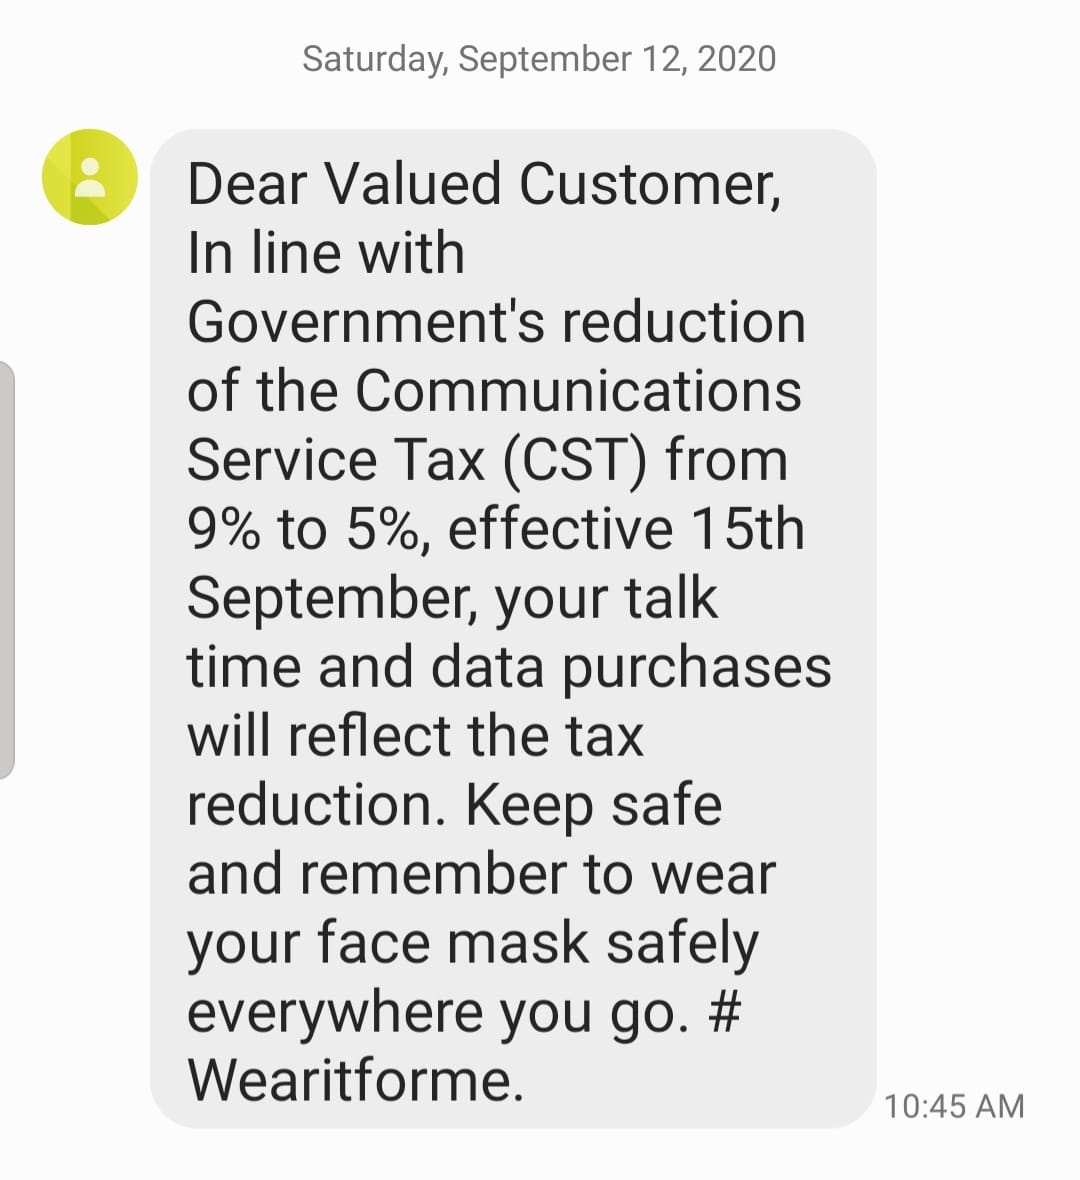
\includegraphics[scale=0.3]{../3-replication-package/original_figures/_commTaxDecrease}}\hspace{1cm}
\includegraphics[scale=0.13]{../3-replication-package/original_figures/_freeZoom}
\end{figure}
}{\large\par}
\par\end{center}

\subsection{Administrative Data -- Motivating Evidence III}
\begin{center}
{\large{}
\begin{figure}[H]
{\large\caption{\textbf{M}{\footnotesize\textbf{OBILE FINANCIAL TRANSACTIONS DURING
COVID-19 }}{\scriptsize\textbf{}}}\label{fig:mobileTransactions}
}{\large\par}
\begin{centering}
{\large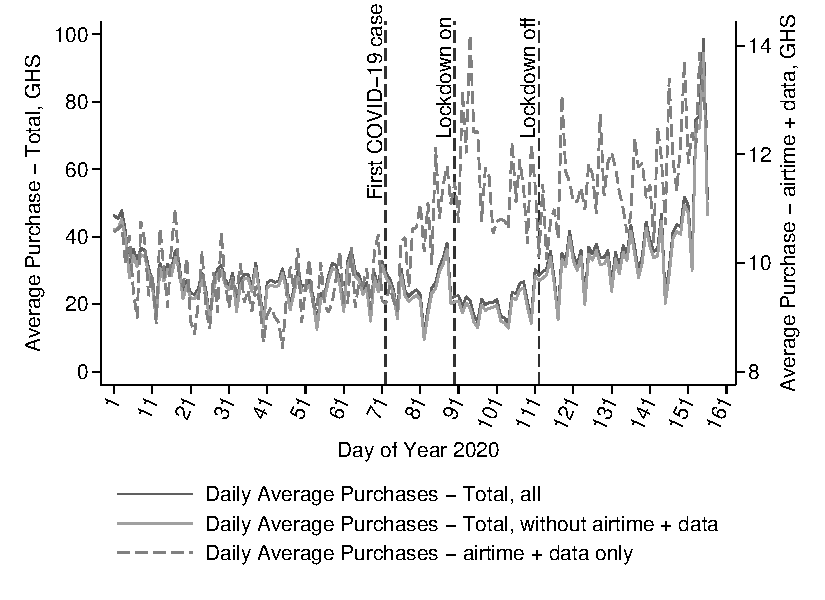
\includegraphics{../3-replication-package/original_figures/mobilefinTransactions}}{\large\par}
\par\end{centering}
\noindent Note: Mobile financial transaction data from a major local
telecommunications company and based on 694,695 transactions (2,0751
random unique subscribers). As displayed, average purchase (total
and total without airtime + data) shown in the left vertical axis
with solid lines, while average purchase for airtime-related activities
(airtime + data only) shown in the right vertical axis with a dash
line. Overall market activity decreased following the onset of the
pandemic, but demand for mobile airtime-related activities sharply
increased over the period. Pre-COVID-19, these two purchases (average
totals versus average airtime) look similar.
\end{figure}
}{\large\par}
\par\end{center}

\end{landscape}

\newpage{}

\subsection{Descriptive Statistics}
\begin{center}
{\large{}
\begin{table}[H]
{\large\caption{\textbf{S}{\footnotesize\textbf{UMMARY STATISTICS OF RELEVANT VARIABLES}}{\large\textbf{
}}{\footnotesize\textbf{}}}\label{tab:summary-baseSurvey-all}
}{\large\par}

\begin{tabular}{lccc}
\hline
Variable & Mean & SD & N \\
\hline\hline
\textbf{Demographic Characteristics} & & & \\ 
Female 0-1 & 0.147 & 0.354 & 1,130 \\ 
Akan ethnic 0-1 & 0.363 & 0.481 & 1,130 \\ 
Married 0-1 & 0.911 & 0.285 & 1,130 \\ 
Attained Junior High School (JHS) 0-1 & 0.784 & 0.412 & 1,130 \\ 
Household size (number) & 6.907 & 4.088 & 1,107 \\ 
Self-employed 0-1 & 0.763 & 0.426 & 1,130 \\ 
Operates in informal sector 0-1 & 0.800 & 0.400 & 1,130 \\ 
Personal income (1 to 5 scale) (monthly) & 1.622 & 0.898 & 1,105 \\ 
Staying together with mother 0-1 (Wave 0) & 0.067 & 0.251 & 1,130 \\ 
Has no religion 0-1 (Wave 0) & 0.054 & 0.226 & 1,130 \\ 
Staying together with spouse 0-1 (Wave 0) & 0.869 & 0.338 & 1,130 \\ 
Age at marriage (Years) (Wave 0) & 24.935 & 4.971 & 1,083 \\ 
\textbf{Poverty} & & & \\ 
Poverty rate (\%) (Schreiner 2005) (Wave 0) & 22.043 & 20.534 & 1,130 \\ 
\textbf{Pandemic Basics} & & & \\ 
Aware of COVID-19 0-1 & 0.996 & 0.060 & 1,105 \\ 
Trust Government's estimates about COVID-19 0-1 & 0.799 & 0.401 & 1,105 \\ 
In previously lockdown region 0-1 & 0.183 & 0.387 & 1,130 \\ 
Self does housework during pandemic 0-1 & 0.168 & 0.374 & 1,105 \\ 
Has relocated / moved in past 7 days 0-1 (Wave 2) & 0.014 & 0.119 & 977 \\ 
\textbf{Key Communication Constraints} & & & \\ 
Need to connect increased due to pandemic 0-1 & 0.701 & 0.458 & 1,104 \\ 
Unable to call in past 7 days 0-1 & 0.627 & 0.484 & 1,103 \\ 
Unable to call due to COVID-19 0-1 & 0.549 & 0.498 & 1,104 \\ 
Unable to make airtime transfers in past 7 days 0-1 & 0.474 & 0.500 & 1,103 \\ 
Borrow airtime 0-1 (Wave 2) & 0.319 & 0.466 & 977 \\ 
Seek digital loan 0-1 (Wave 2) & 0.088 & 0.283 & 977 \\ 
\textbf{Well-being Measures} & & & \\ 
Total Expenditure (GHS) (weekly) & 324.112 & 423.254 & 1,102 \\ 
Threatened Partner (1 = never to 4 = very often) & 1.194 & 0.701 & 1,102 \\ 
Hit Partner (1 = never to 4 = very often) & 1.134 & 0.670 & 1,102 \\ 
log K10 & 2.820 & 0.369 & 1,102 \\ 
Severe Distress 0-1 & 0.096 & 0.295 & 1,102 \\ 
I'm tired (mentally, emotionally, or socially) of COVID-19 0-1 & 0.539 & 0.499 & 1,104 \\ 
I'm depressed (1 = disagree to 5 = agree) & 1.600 & 0.942 & 1,102 \\ 
I'm relaxed (1 = disagree to 5 = agree) & 2.885 & 1.384 & 1,102 \\ 
I'm satisfied with life, all else equal (1 = disagree to 5 = agree) & 2.536 & 1.318 & 1,102 \\ 
I'm satisfied with finances, all else equal (1 = disagree to 5 = agree) & 2.074 & 1.157 & 1,102 \\ 
\hline\hline
\end{tabular}


\begin{spacing}{0.8}
Note: Observations are at the individual level. Table reports the
summary statistics of relevant variables from our baseline survey
waves. This include information about demographics, poverty indicators,
communication and well-being outcomes, respectively. The exchange
rate during the baseline period is US\$ 1.0 = GHS 5.80.
\end{spacing}
\end{table}
}{\large\par}
\par\end{center}

\begin{center}
{\large{}
\begin{figure}[H]
{\large\caption{\textbf{K}{\footnotesize\textbf{ 10 SCORE}}{\scriptsize\textbf{ AT
BASELINE (WAVE 1)}}}\label{fig:subjects_k10_base}
}{\large\par}
\begin{centering}
{\large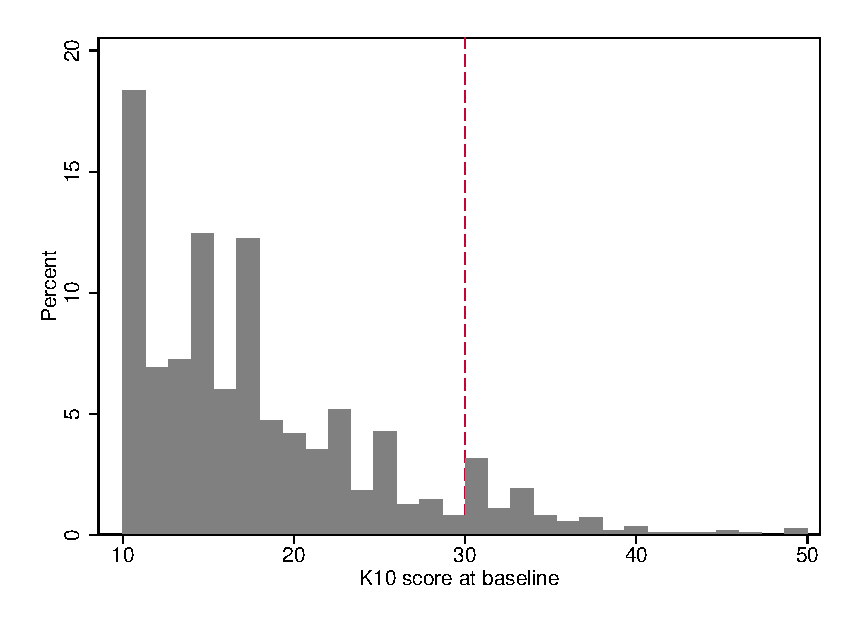
\includegraphics[scale=0.65]{../3-replication-package/Output/Figures/figure_a3}}{\large\par}
\par\end{centering}
Note: Observations are at the individual level. Low (scores of 10-15,
indicating little or no psychological distress). Moderate (scores
of 16-21). High (scores of 22-29). Very high or severe distress (scores
of 30-50). 11.5\% rate of severe distress (indicated by the vertical
dashed line).
\end{figure}
}{\large\par}
\par\end{center}

\begin{center}
{\large{}
\begin{figure}[H]
{\large\caption{\textbf{T}{\footnotesize\textbf{OTAL CONSUMPTION EXPENDITURE }}{\scriptsize\textbf{AT
BASELINE (WAVE 1)}}}\label{fig:subjects_totconsump_base}
}{\large\par}
\begin{centering}
{\large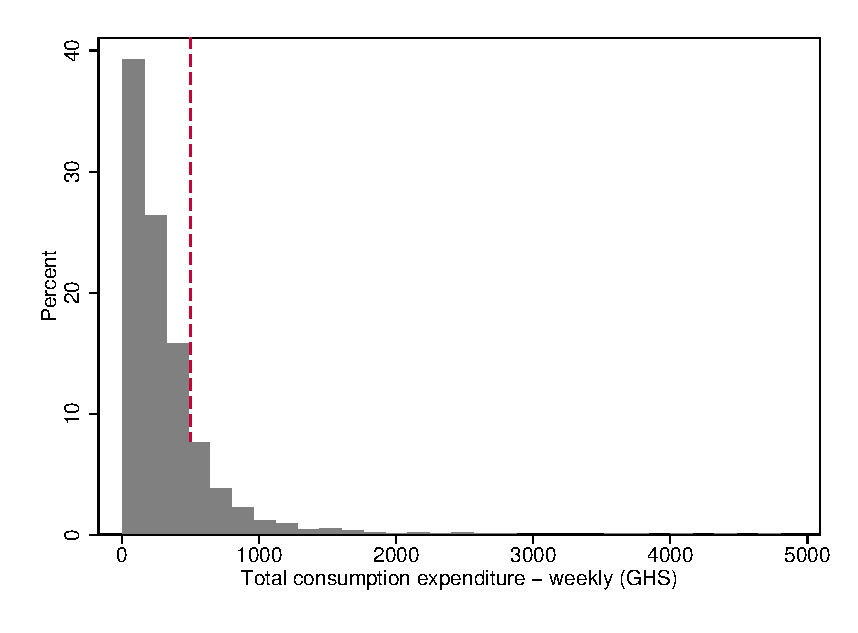
\includegraphics[scale=0.65]{../3-replication-package/Output/Figures/figure_a4}}{\large\par}
\par\end{centering}
Note: Observations are at the individual level. Total consumption
expenditure sums all expenses: food (inside and outside home), utilities,
personal care, education, health, and durables. 81.7\% rate of poor
consumption ($\leq$ 500GHS per week and indicated by the dashed vertical
line).
\end{figure}
}{\large\par}
\par\end{center}

\newpage{}

\subsection{Balance}
\begin{center}
{\large{}
\begin{table}[H]
{\large\caption{\textbf{B}{\footnotesize\textbf{ALANCE TEST: PRE-INTERVENTION TREATMENT-CONTROL
DIFFERENCES }}}\label{tab:treatment_balanceY}
}{\large\par}

\include{../3-replication-package/Output/Tables/Table_a4}

\begin{spacing}{0.7}
Note: Observations are at the individual level. Each row is a separate
regression. Clustered standard errors (at the district level) are
reported in parentheses. {*}{*}{*} p<0.01, {*}{*} p<0.05, {*} p<0.10.
Mean baseline characteristics are also balanced across treatment arms.
\textbf{Results are similar with and without controls for randomization
strata dummies.}
\end{spacing}
\end{table}
}{\large\par}
\par\end{center}

\begin{center}
{\large{}
\begin{table}[H]
{\large\caption{\textbf{B}{\footnotesize\textbf{ALANCE TEST: PRE-INTERVENTION TREATMENT-CONTROL
DIFFERENCES }}}\label{tab:treatment_balanceXs}
}{\large\par}

\include{../3-replication-package/Output/Tables/Table_a5}

\begin{spacing}{0.7}
Note: Observations are at the individual level. Each row is a separate
regression. The F and Chi-squared tests are conducted using the pooled
indicator \textbf{1(Communication Credit)} as the outcome and excluding
all the communication and well-being outcomes. Clustered standard
errors (at the district level) are reported in parentheses. {*}{*}{*}
p<0.01, {*}{*} p<0.05, {*} p<0.10. Mean baseline characteristics are
also balanced across treatment arms. \textbf{Results are similar with
and without controls for randomization strata dummies.}
\end{spacing}
\end{table}
}{\large\par}
\par\end{center}

\begin{center}
{\large{}
\begin{figure}[H]
{\large\caption{\textbf{P}{\footnotesize\textbf{HONE CALLS AND REACHABILITY OF INDIVIDUALS}}{\scriptsize\textbf{}}}\label{fig:subjects_reachability}
}{\large\par}
\centering{}{\large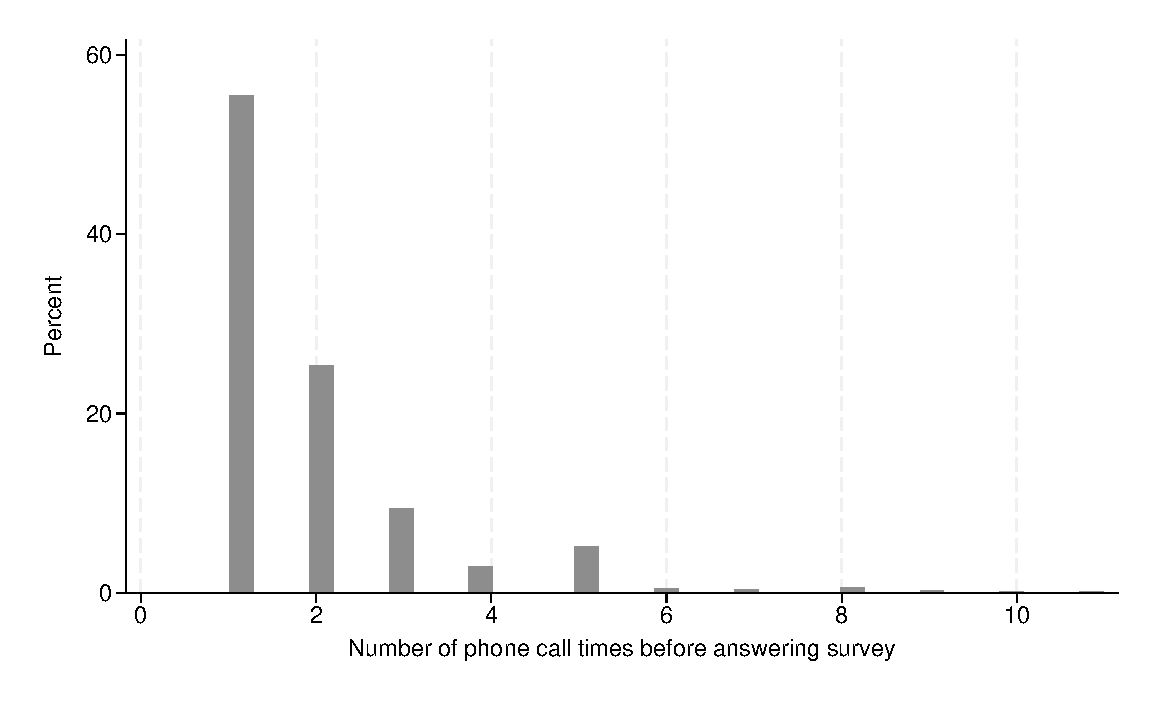
\includegraphics[scale=0.65]{../3-replication-package/Output/Figures/figure_a5}}{\large\par}
\end{figure}
}{\large\par}
\par\end{center}

\newpage{}
\begin{doublespace}

\subsection{Further Results -- Tables and Figures}
\end{doublespace}
\begin{center}
\textbf{POOLED EFFECTS OVER TRAJECTORY}
\par\end{center}

\begin{center}
{\large{}
\begin{figure}[H]
{\large\caption{{\footnotesize\textbf{MITIGATION OF COMMUNICATION CONSTRAINTS }}{\scriptsize\textbf{}}}\label{fig:mitigate_trajectory_meta}
}{\large\par}
\begin{centering}
{\large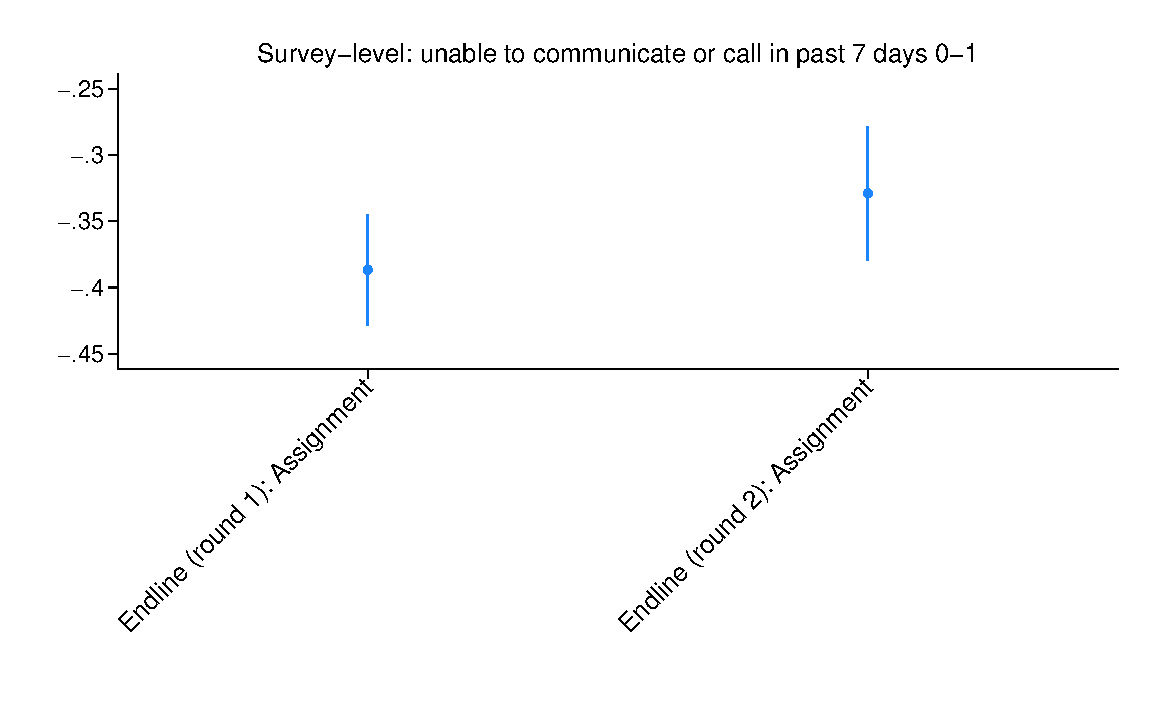
\includegraphics[scale=0.55]{../3-replication-package/Output/Figures/figure_a6_1}...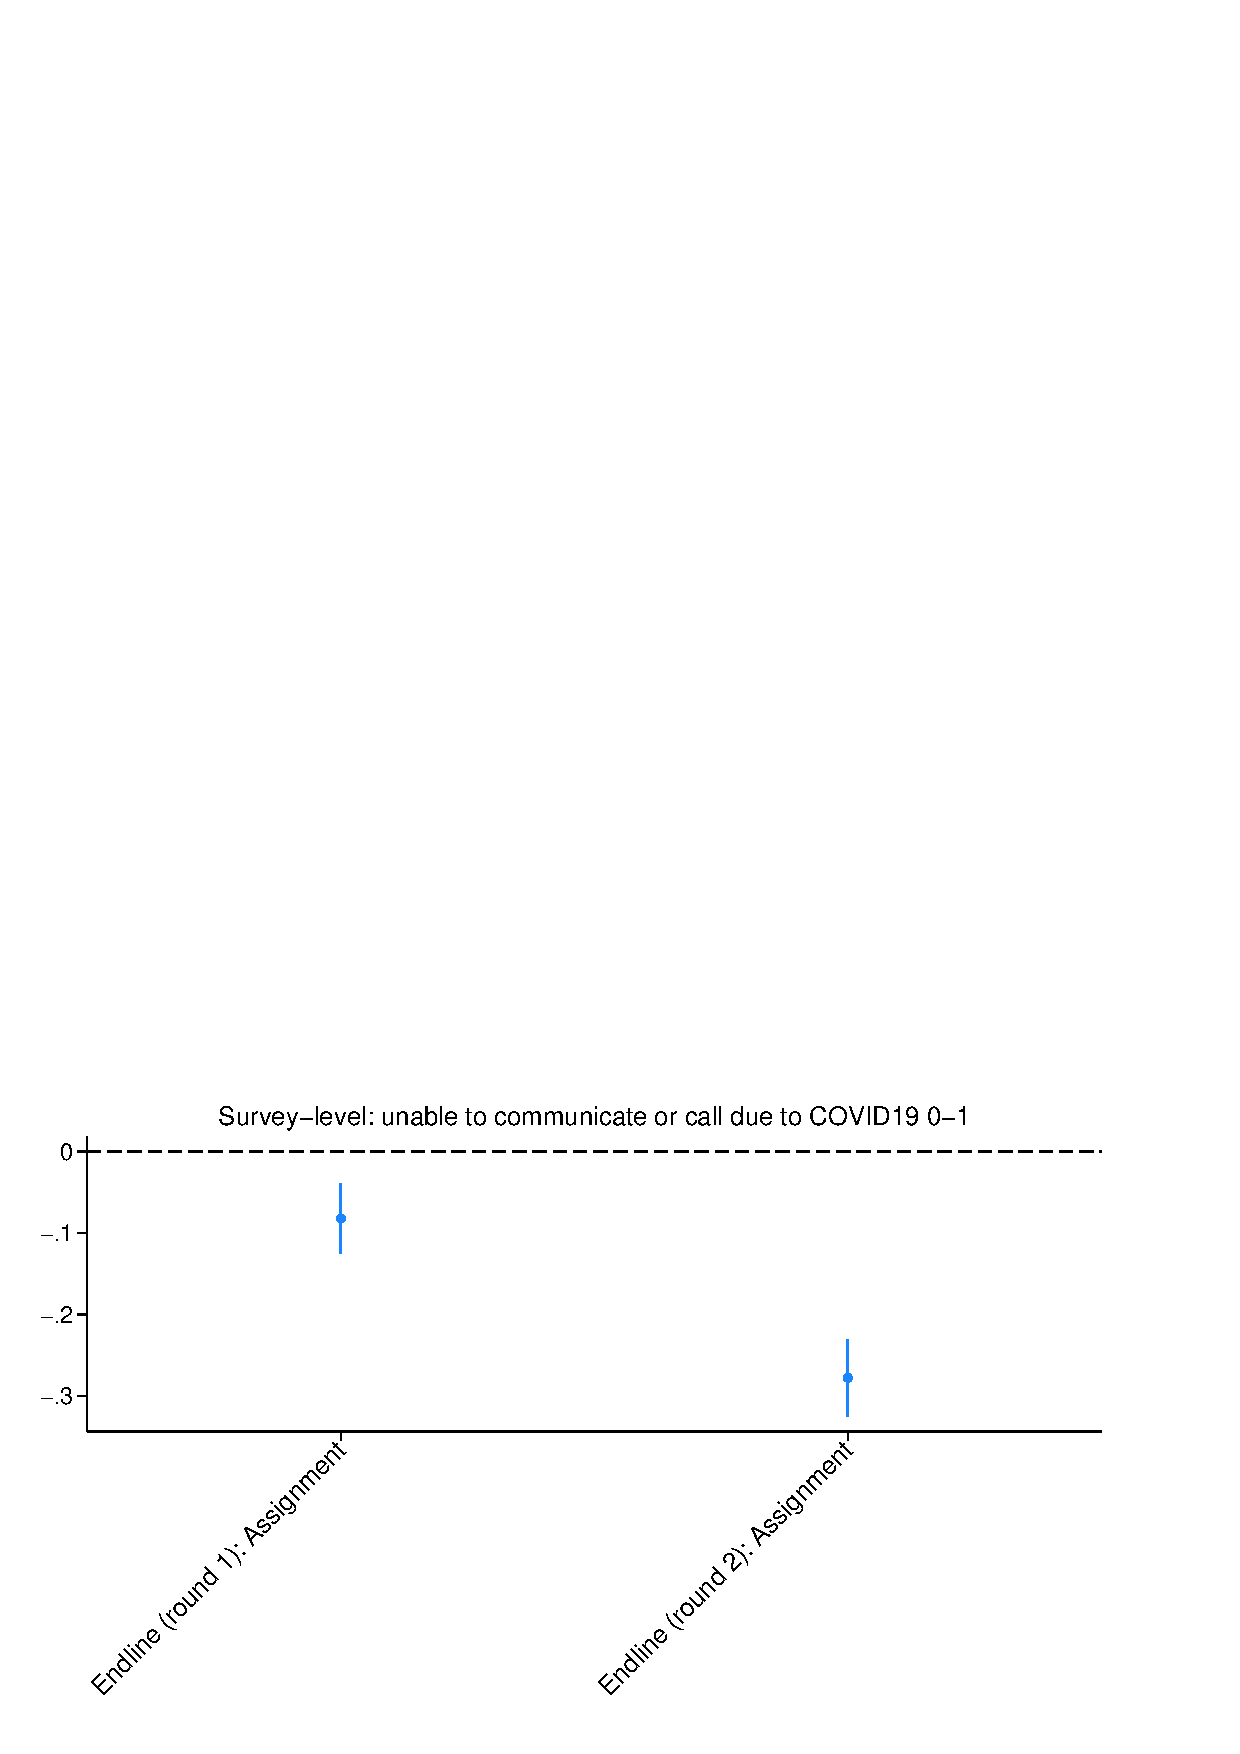
\includegraphics[scale=0.55]{../3-replication-package/Output/Figures/figure_a6_2}}\\
{\large\par}
\par\end{centering}
\begin{centering}
{\large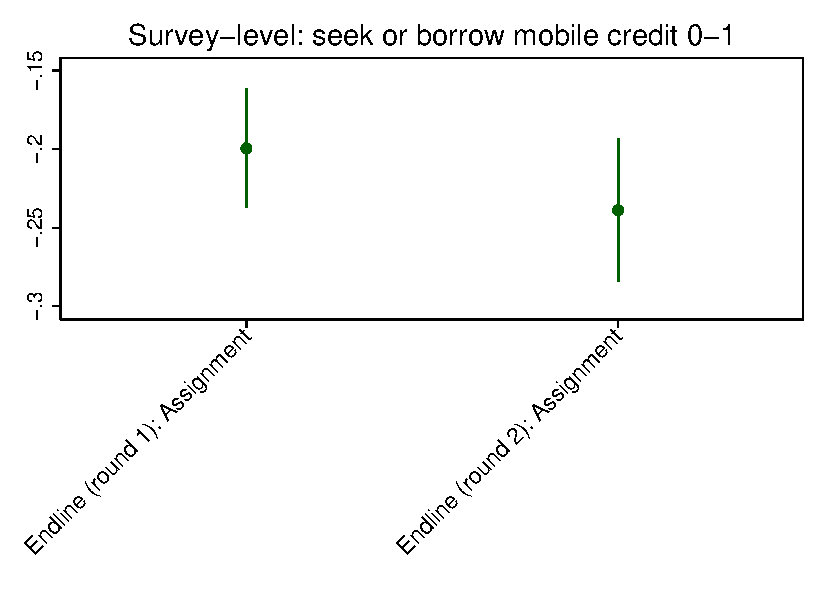
\includegraphics[scale=0.55]{../3-replication-package/Output/Figures/figure_a6_3}...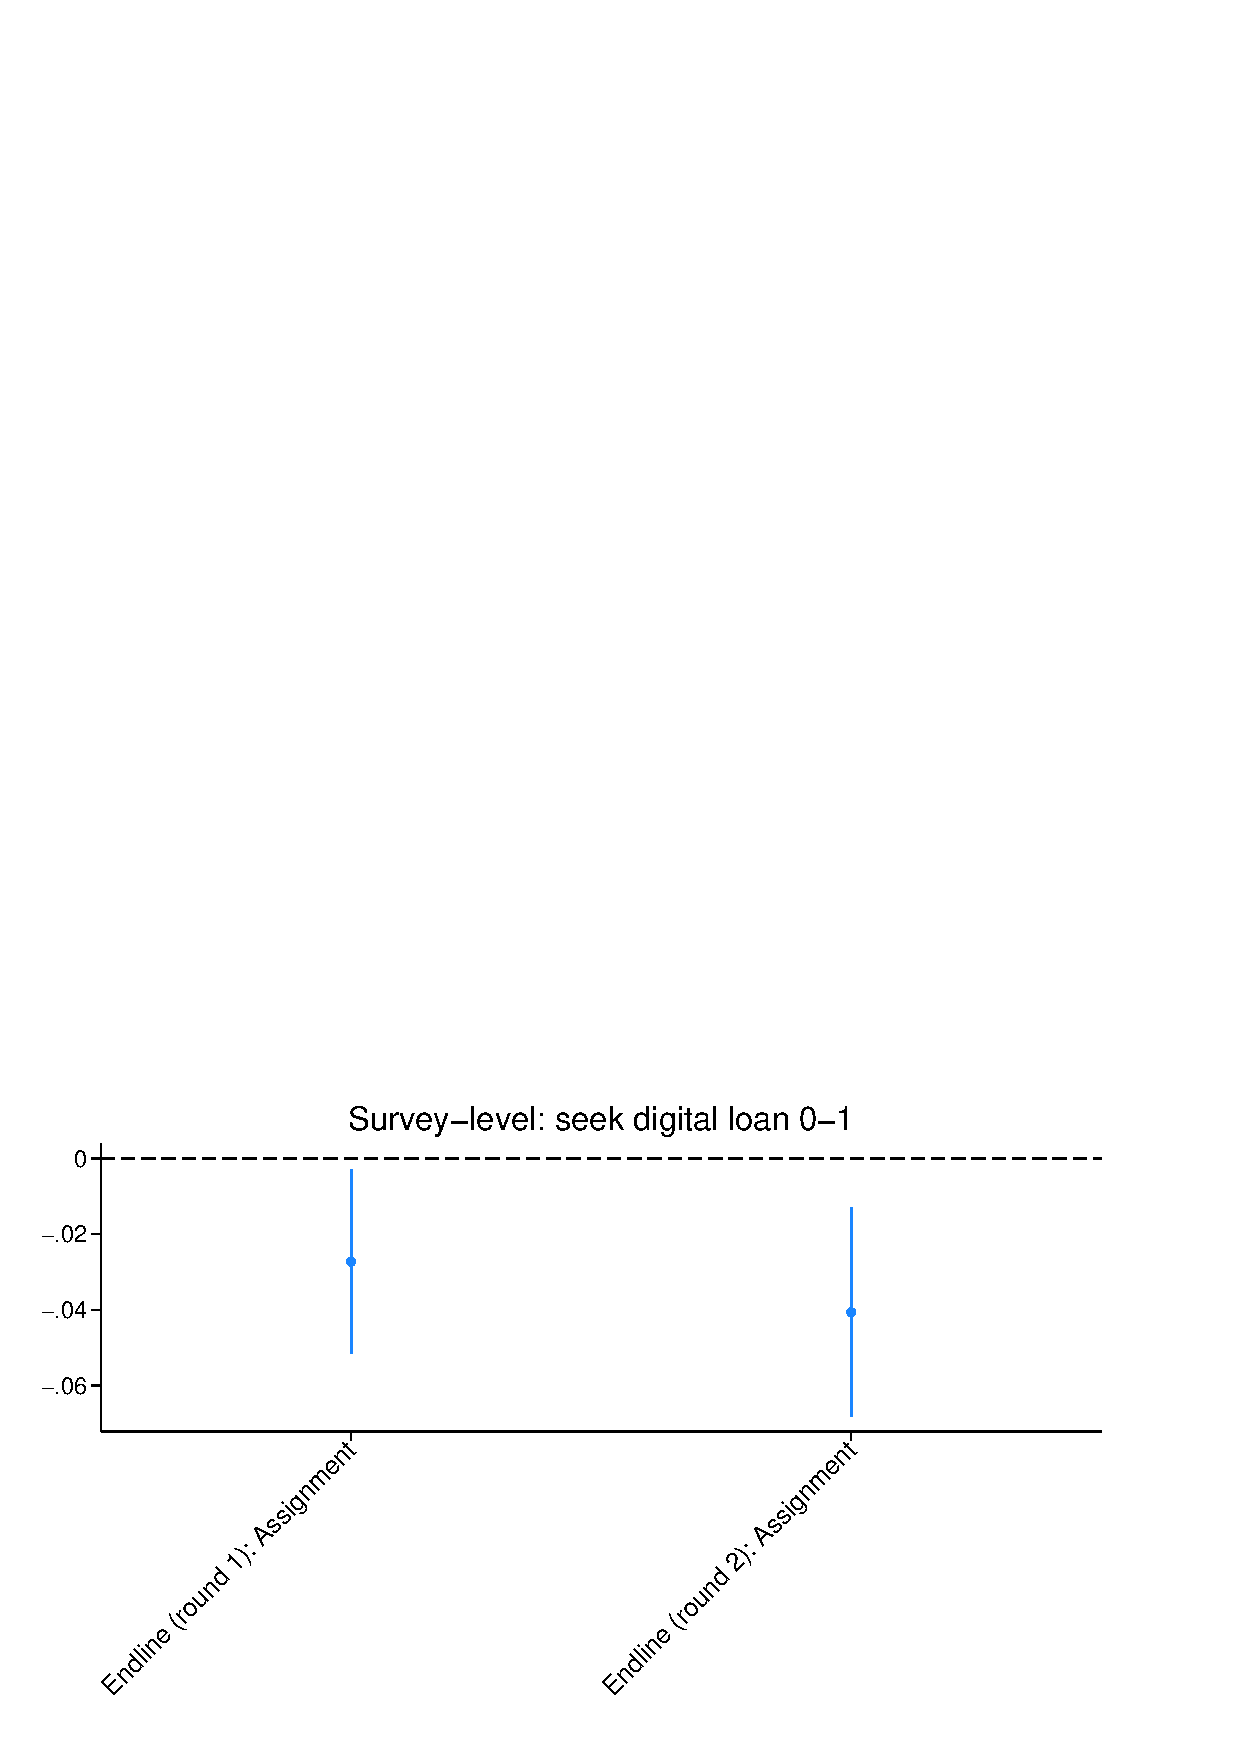
\includegraphics[scale=0.55]{../3-replication-package/Output/Figures/figure_a6_4}}{\large\par}
\par\end{centering}
{\large\vspace*{0.2cm}
}Note: Estimates are from a model that includes randomization strata
(district) fixed effects, survey date fixed effects, and double-post
LASSO specification which considers all individual controls, and individual
district and survey date fixed effects in the possible control set.
Controls include: individual’s age, 0-1 indicator for whether married
or not, 0-1 indicator for whether belongs to akan ethnic group or
not, 0-1 indicator for whether self employed or not, household size,
0-1 indicator for whether operates in the informal sector, monthly
personal income over an ordinal scale of 1 to 5, 0-1 indicator for
whether attained junior high school (JHS) education, and individual’s
gender. Observations are at the subject $\times$ date level. Standard
errors are clustered at the individual level (the level of treatment).
90\% confidence intervals are displayed around the estimates. Table
of coefficients and standard errors available upon request.
\end{figure}
}{\large\par}
\par\end{center}

\begin{center}
{\large{}
\begin{figure}[H]
{\large\caption{{\footnotesize\textbf{IMPACTS OF COMMUNICATION PROGRAMS ON WELL-BEING
MEASURES }}{\scriptsize\textbf{}}}\label{fig:consumpxhealth_trajectory_meta}
}{\large\par}
\begin{centering}
{\large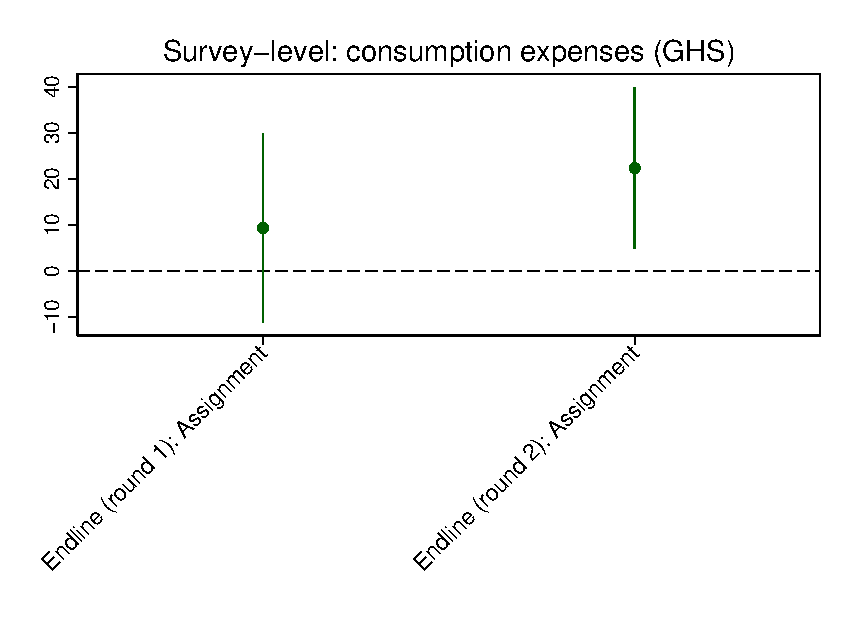
\includegraphics[scale=0.5]{../3-replication-package/Output/Figures/figure_a7_1}...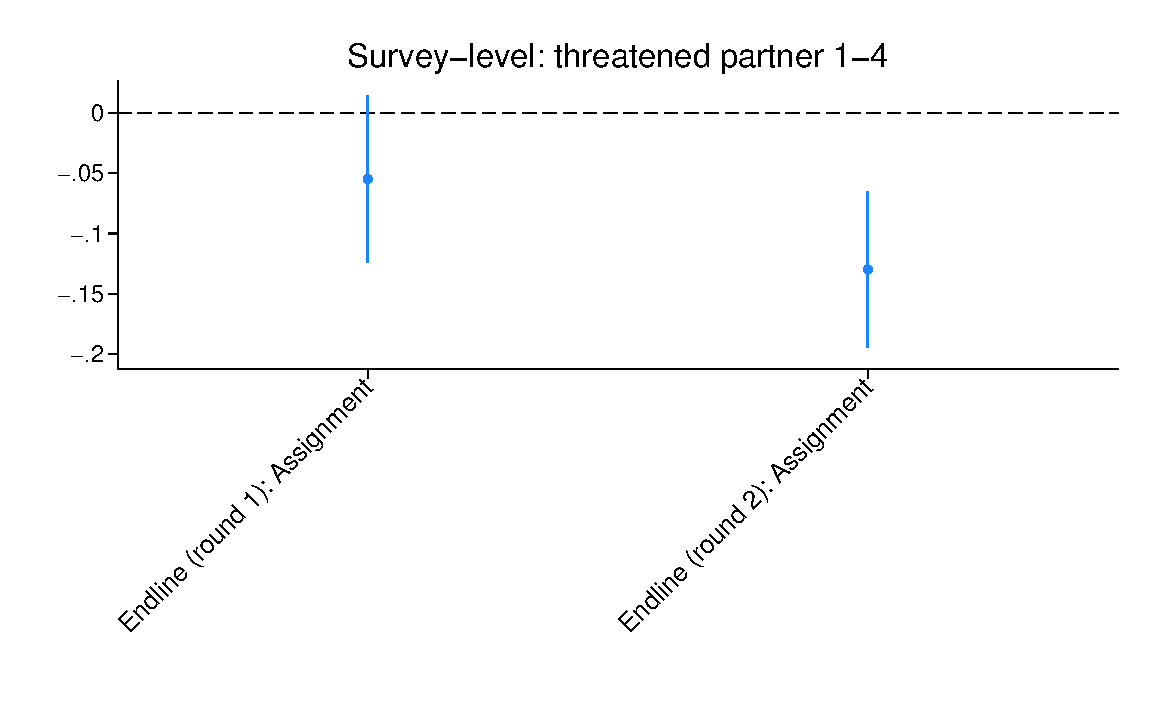
\includegraphics[scale=0.5]{../3-replication-package/Output/Figures/figure_a7_2}}{\small}\\
{\small\par}
\par\end{centering}
\begin{centering}
{\large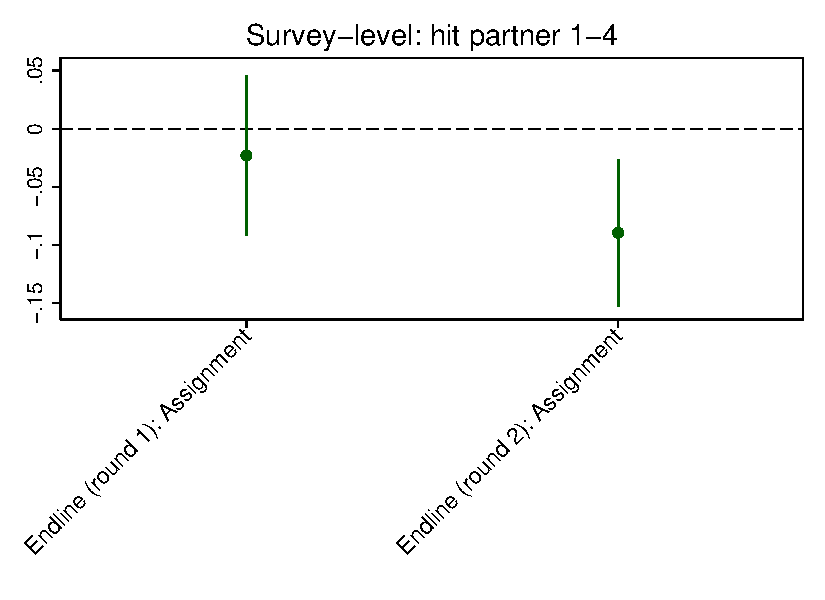
\includegraphics[scale=0.55]{../3-replication-package/Output/Figures/figure_a7_3}}\\
{\large\par}
\par\end{centering}
\begin{centering}
{\large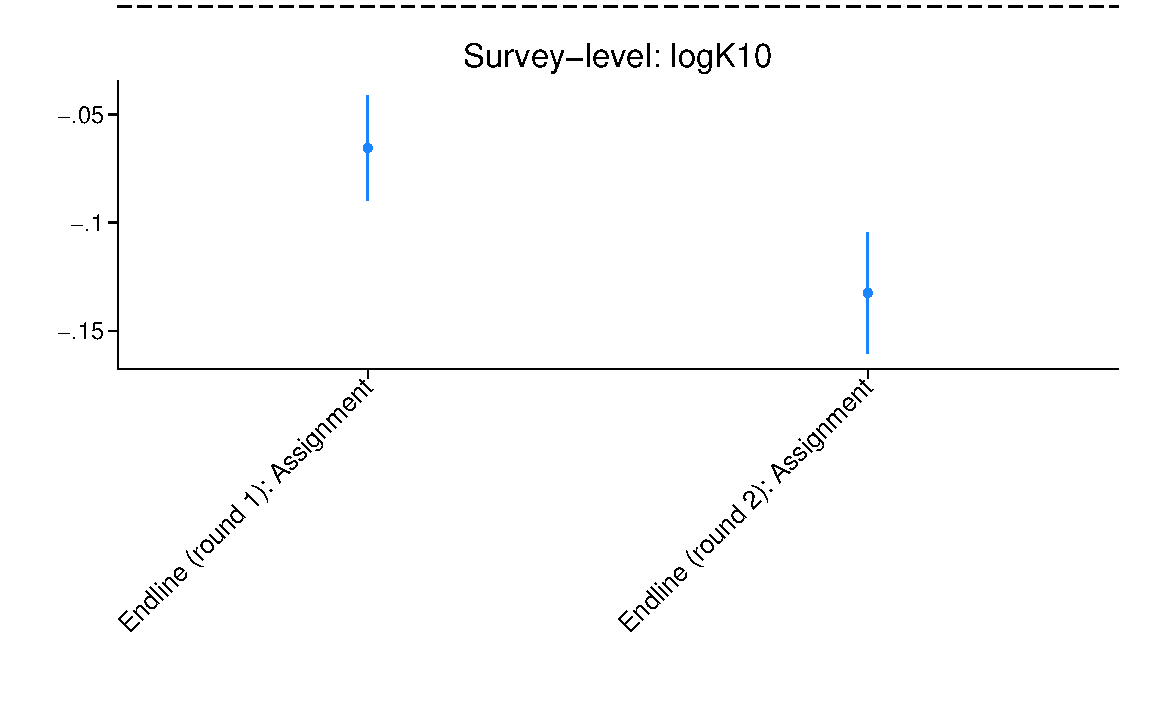
\includegraphics[scale=0.5]{../3-replication-package/Output/Figures/figure_a7_4}...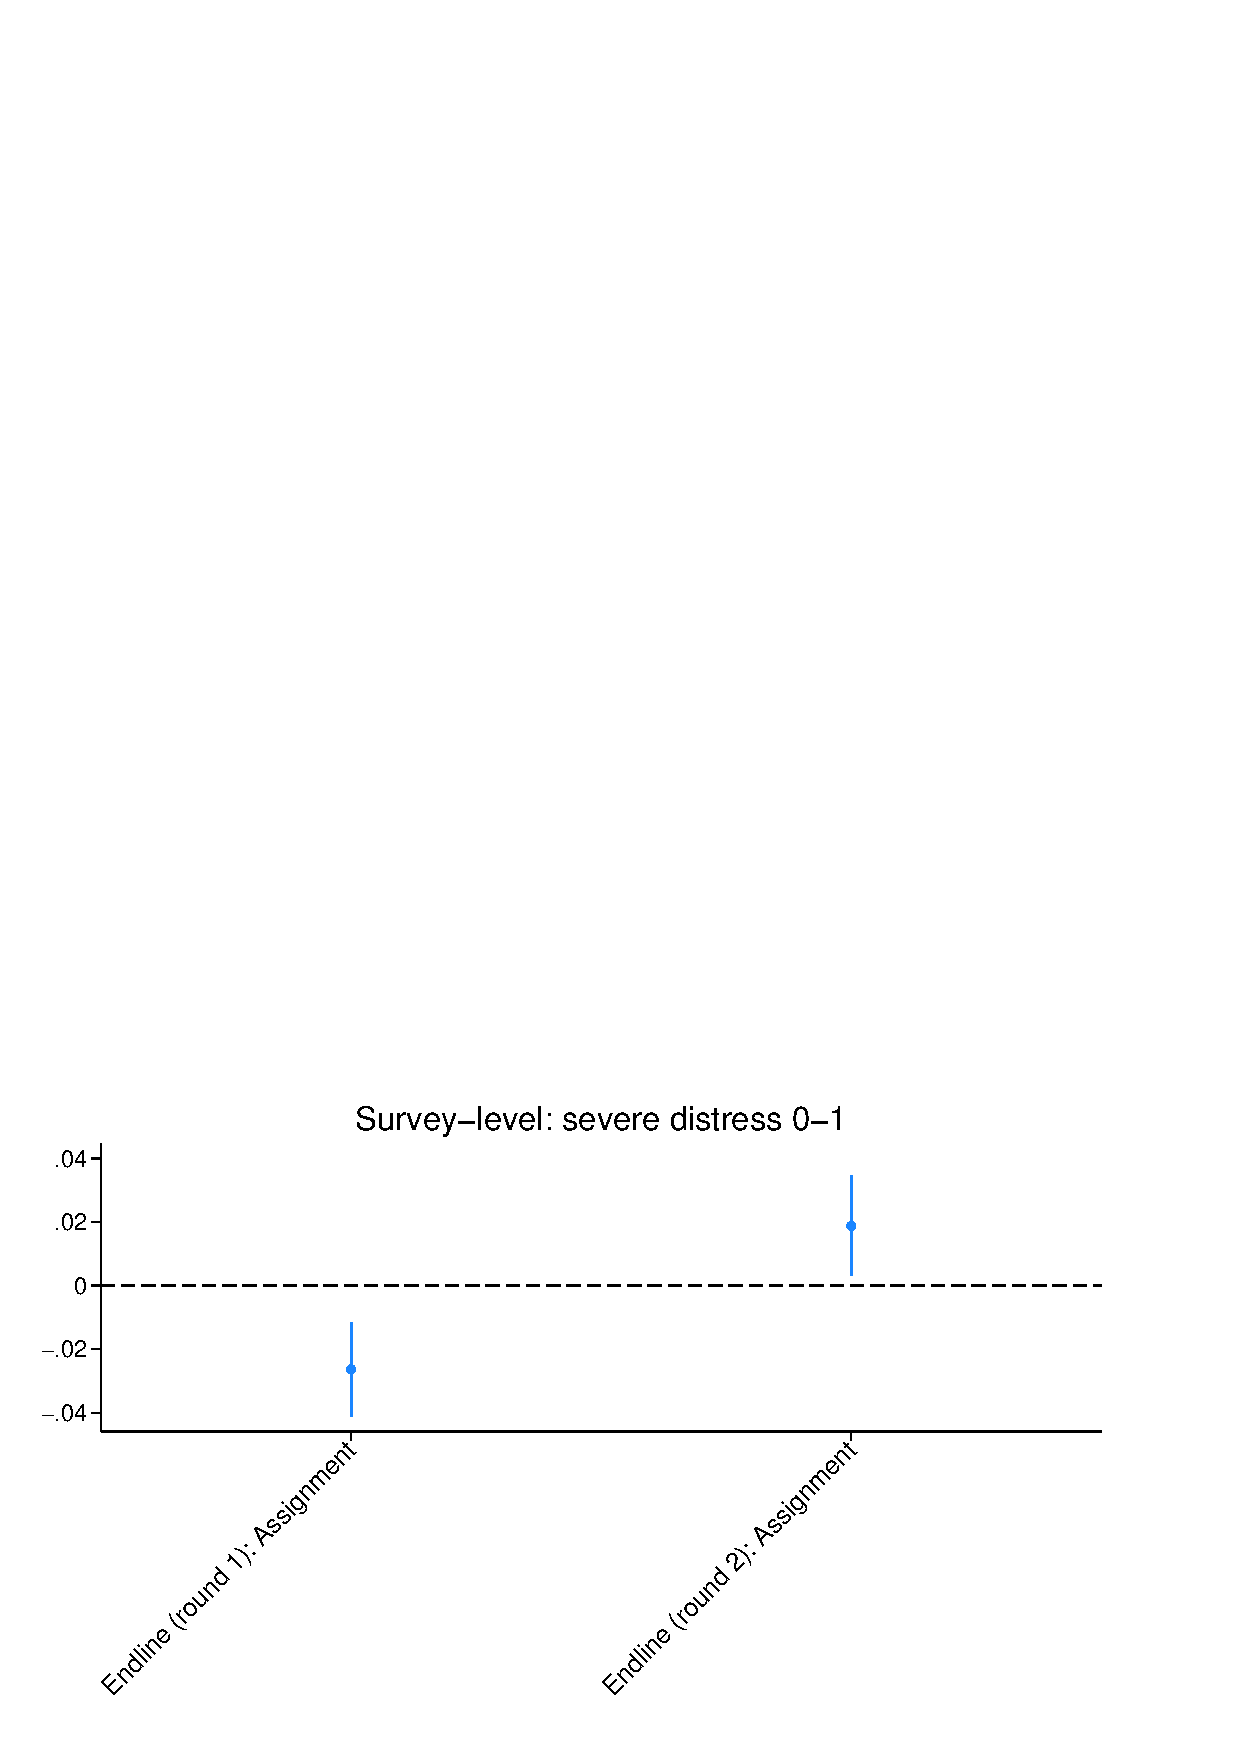
\includegraphics[scale=0.5]{../3-replication-package/Output/Figures/figure_a7_5}}{\large\par}
\par\end{centering}
{\large\vspace*{0.2cm}
}Note: Estimates are from a model that includes randomization strata
(district) fixed effects, survey date fixed effects, and double-post
LASSO specification which considers all individual controls, and individual
district and survey date fixed effects in the possible control set.
Controls include: individual’s age, 0-1 indicator for whether married
or not, 0-1 indicator for whether belongs to akan ethnic group or
not, 0-1 indicator for whether self employed or not, household size,
0-1 indicator for whether operates in the informal sector, monthly
personal income over an ordinal scale of 1 to 5, 0-1 indicator for
whether attained junior high school (JHS) education, and individual’s
gender. Observations are at the subject $\times$ date level. Standard
errors are clustered at the individual level (the level of treatment).
90\% confidence intervals are displayed around the estimates. Table
of coefficients and standard errors available upon request.
\end{figure}
}{\large\par}
\par\end{center}

\newpage{}
\begin{center}
\textbf{SEPARATE EFFECTS OVER TRAJECTORY}
\par\end{center}

\begin{center}
{\large{}
\begin{figure}[H]
{\large\caption{{\footnotesize\textbf{MITIGATION OF COMMUNICATION CONSTRAINTS }}{\scriptsize\textbf{}}}\label{fig:mitigate_trajectory_sep}
}{\large\par}
\begin{centering}
{\large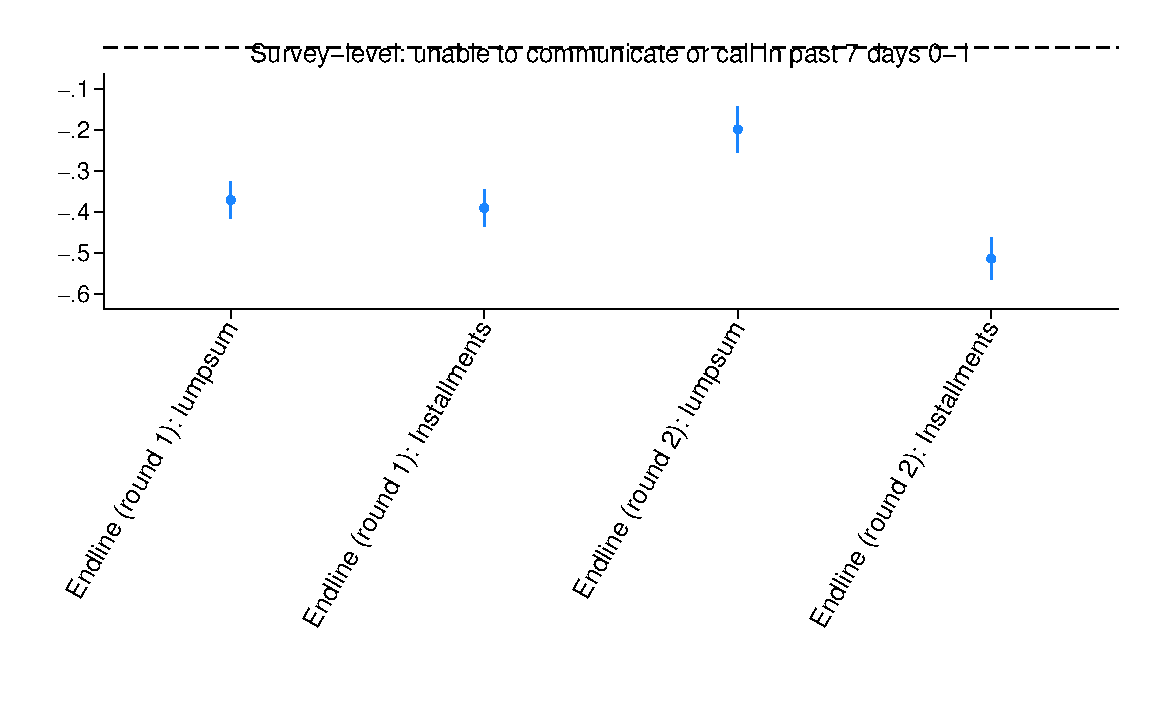
\includegraphics[scale=0.55]{../3-replication-package/Output/Figures/figure_a8_1}...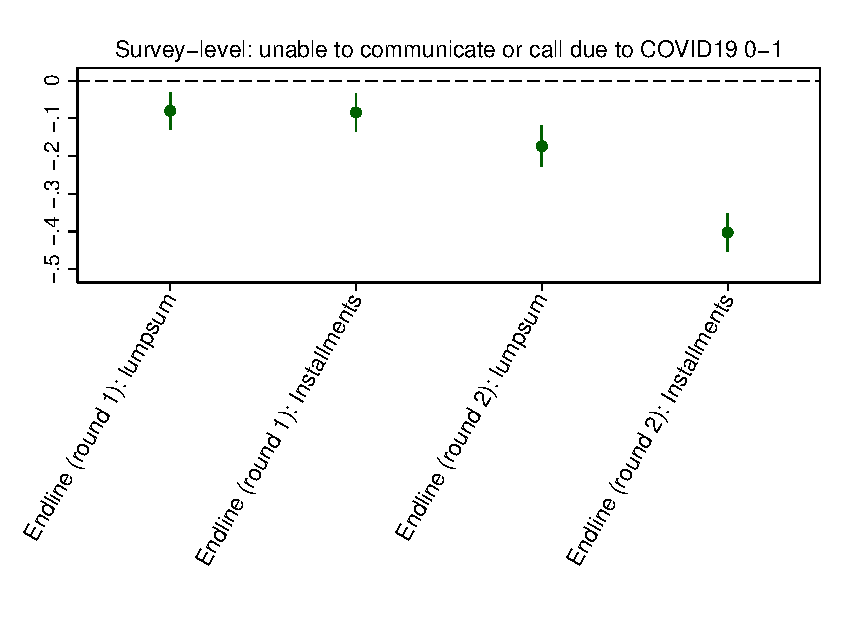
\includegraphics[scale=0.55]{../3-replication-package/Output/Figures/figure_a8_2}}\\
{\large\par}
\par\end{centering}
\begin{centering}
{\large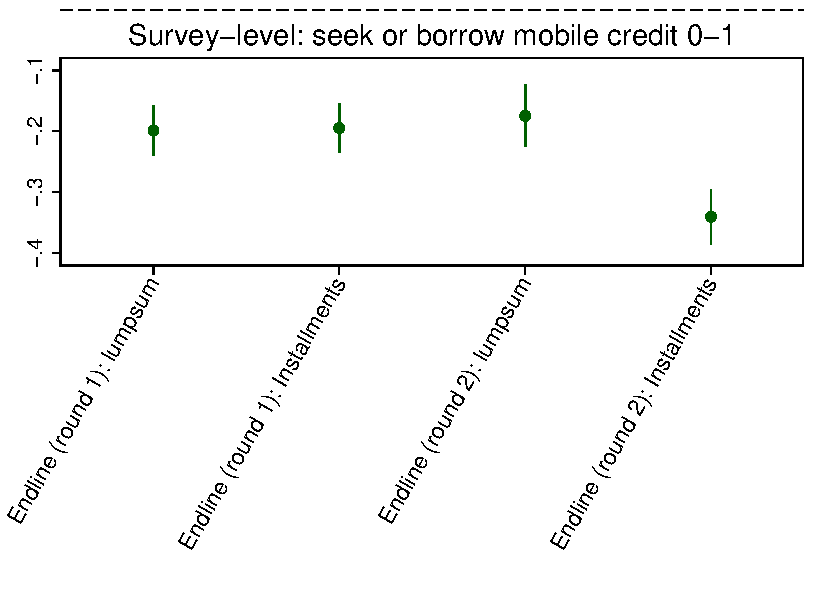
\includegraphics[scale=0.55]{../3-replication-package/Output/Figures/figure_a8_3}...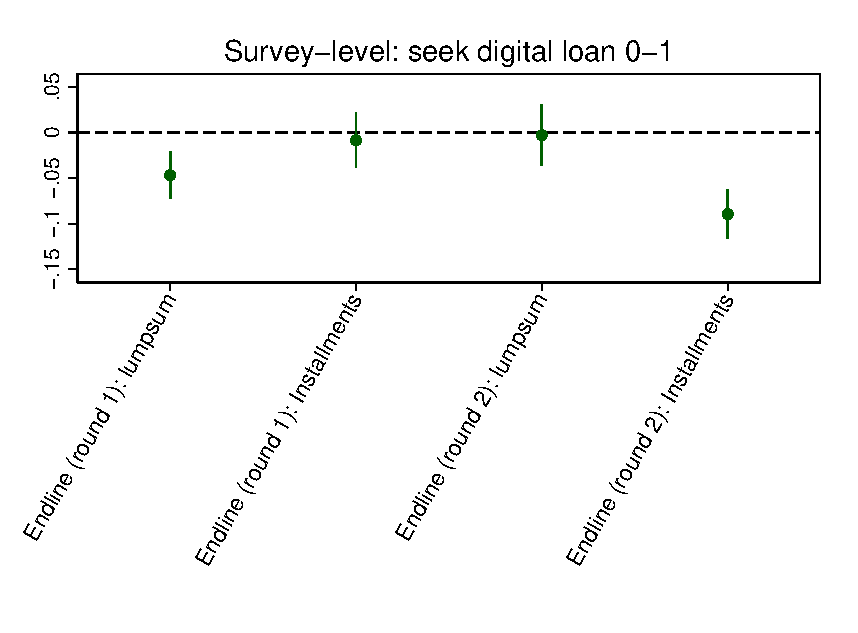
\includegraphics[scale=0.55]{../3-replication-package/Output/Figures/figure_a8_4}}{\large\par}
\par\end{centering}
{\large\vspace*{0.2cm}
}Note: Estimates are from a model that includes randomization strata
(district) fixed effects, survey date fixed effects, and double-post
LASSO specification which considers all individual controls, and individual
district and survey date fixed effects in the possible control set.
Controls include: individual’s age, 0-1 indicator for whether married
or not, 0-1 indicator for whether belongs to akan ethnic group or
not, 0-1 indicator for whether self employed or not, household size,
0-1 indicator for whether operates in the informal sector, monthly
personal income over an ordinal scale of 1 to 5, 0-1 indicator for
whether attained junior high school (JHS) education, and individual’s
gender. Observations are at the subject $\times$ date level. Standard
errors are clustered at the individual level (the level of treatment).
90\% confidence intervals are displayed around the estimates. Table
of coefficients and standard errors available upon request.
\end{figure}
}{\large\par}
\par\end{center}

\begin{center}
{\large{}
\begin{figure}[H]
{\large\caption{{\footnotesize\textbf{IMPACTS OF COMMUNICATION PROGRAMS ON WELL-BEING}}{\scriptsize\textbf{}}}\label{fig:consumpxhealth_trajectory_sep}
}{\large\par}
\begin{centering}
{\large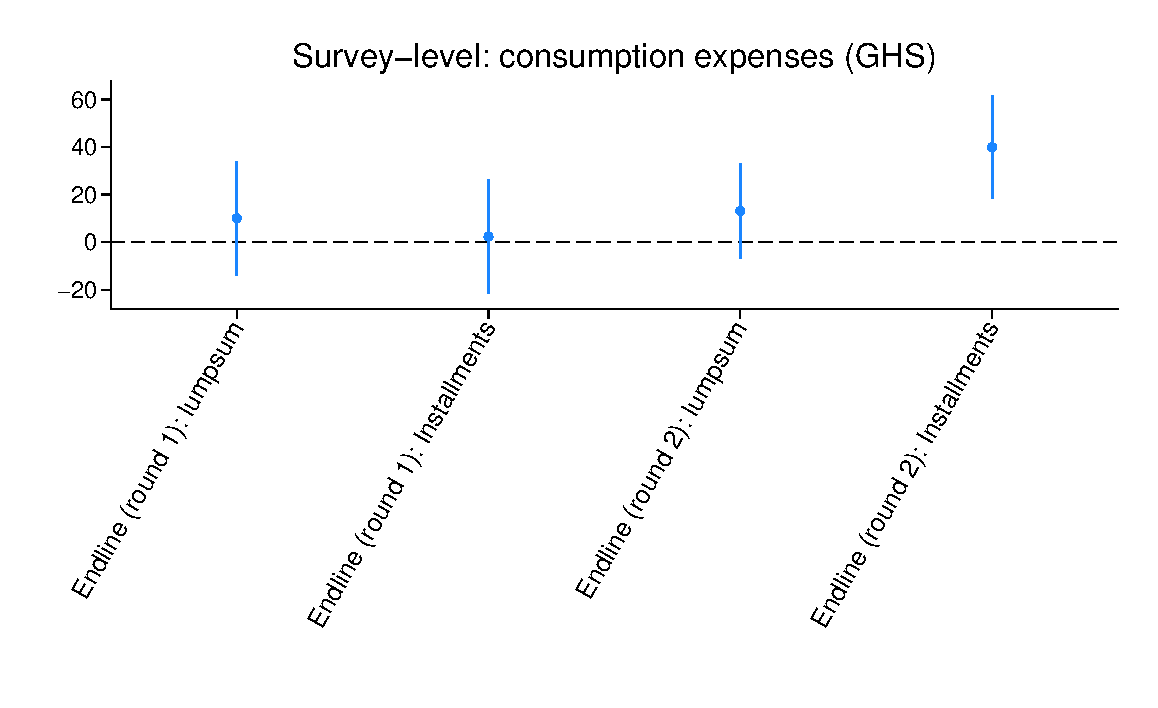
\includegraphics[scale=0.5]{../3-replication-package/Output/Figures/figure_a9_1}...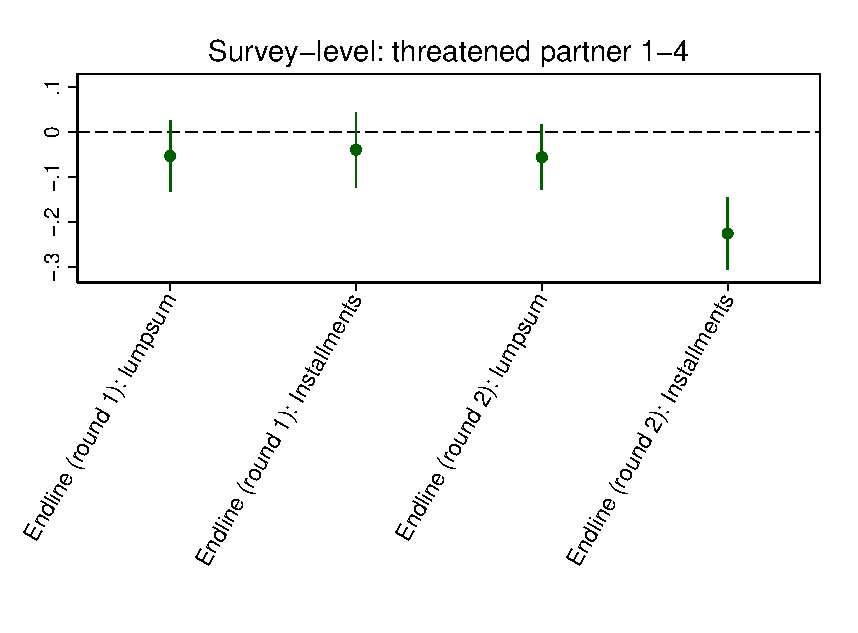
\includegraphics[scale=0.5]{../3-replication-package/Output/Figures/figure_a9_2}}{\small}\\
{\small\par}
\par\end{centering}
\begin{centering}
{\large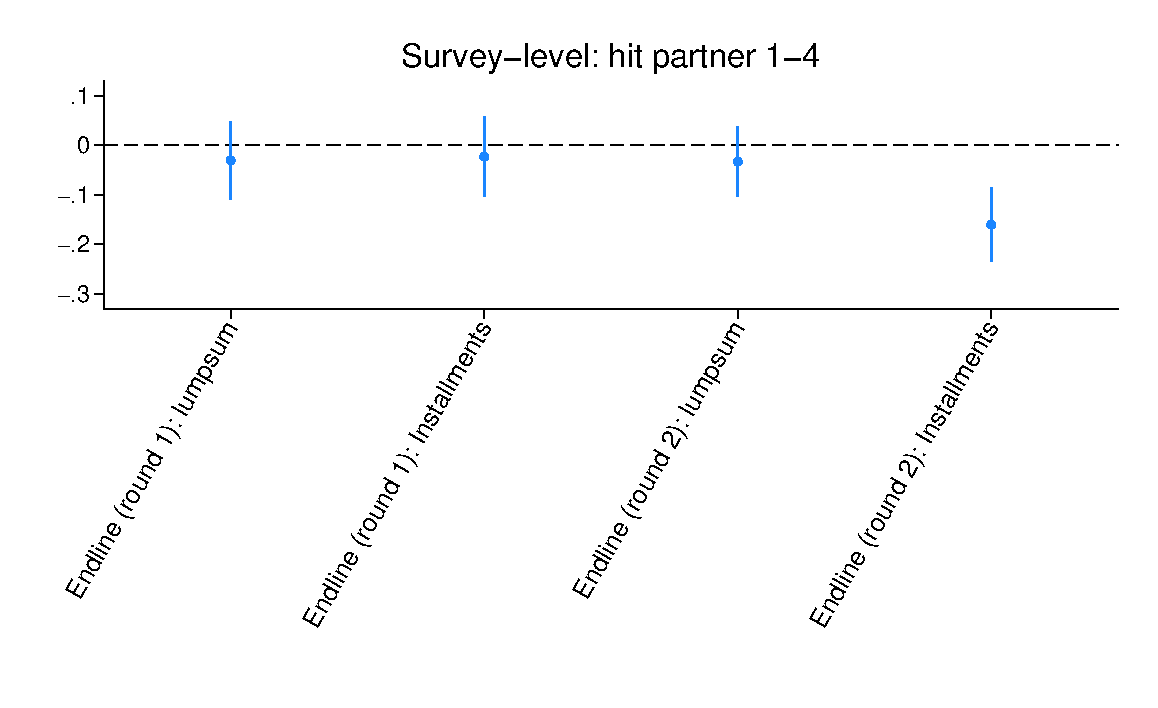
\includegraphics[scale=0.55]{../3-replication-package/Output/Figures/figure_a9_3}}\\
{\large\par}
\par\end{centering}
\begin{centering}
{\large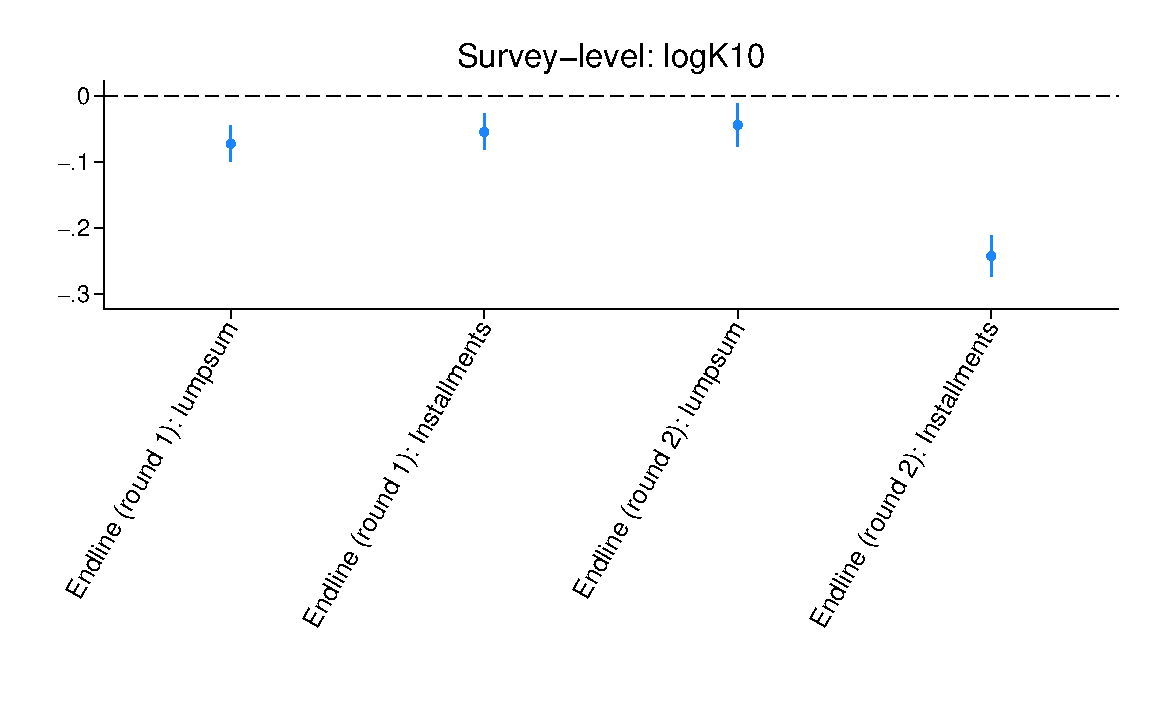
\includegraphics[scale=0.5]{../3-replication-package/Output/Figures/figure_a9_4}...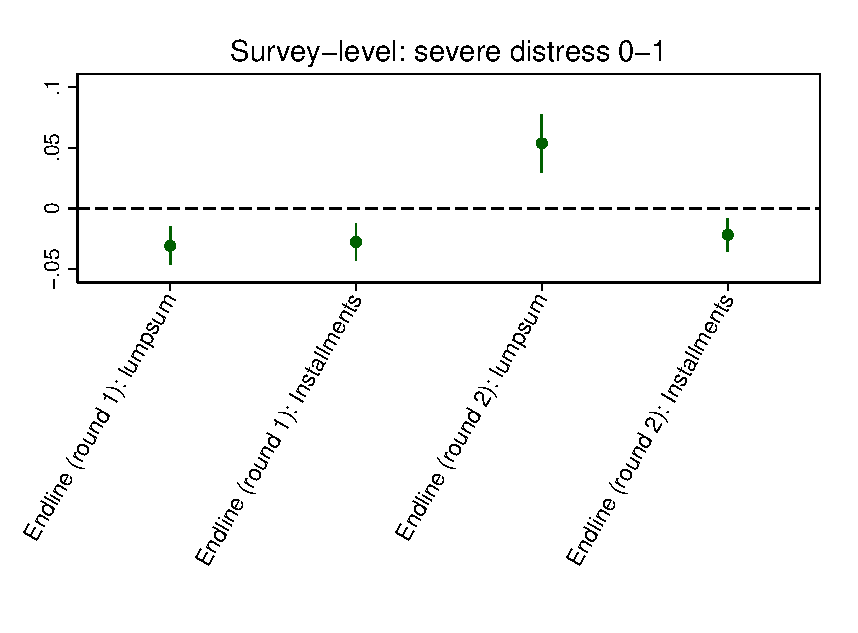
\includegraphics[scale=0.5]{../3-replication-package/Output/Figures/figure_a9_5}}{\large\par}
\par\end{centering}
{\large\vspace*{0.2cm}
}Note: Estimates are from a model that includes randomization strata
(district) fixed effects, survey date fixed effects, and double-post
LASSO specification which considers all individual controls, and individual
district and survey date fixed effects in the possible control set.
Controls include: individual’s age, 0-1 indicator for whether married
or not, 0-1 indicator for whether belongs to akan ethnic group or
not, 0-1 indicator for whether self employed or not, household size,
0-1 indicator for whether operates in the informal sector, monthly
personal income over an ordinal scale of 1 to 5, 0-1 indicator for
whether attained junior high school (JHS) education, and individual’s
gender. Observations are at the subject $\times$ date level. Standard
errors are clustered at the individual level (the level of treatment).
90\% confidence intervals are displayed around the estimates. Table
of coefficients and standard errors available upon request.
\end{figure}
}{\large\par}
\par\end{center}

\newpage{}

\noindent\begin{landscape}
\begin{center}
\textbf{HETEROGENEOUS EFFECTS}
\par\end{center}

\begin{center}
\begin{table}
\caption{\textbf{I}{\footnotesize\textbf{MPACTS OF COMMUNICATION PROGRAMS ON
WELL-BEING BY POVERTY }}}\label{tab:wellbeingXpoverty_pooled_meta}

\include{../3-replication-package/Output/Tables/Table_a6}

{\large\vspace*{0.2cm}
}Note: District is the randomization strata. The double-post LASSO
specification considers all individual controls, and individual district
and survey date fixed effects in the possible control set. Controls
include: individual’s age, 0-1 indicator for whether married or not,
0-1 indicator for whether belongs to akan ethnic group or not, 0-1
indicator for whether self employed or not, household size, 0-1 indicator
for whether operates in the informal sector, monthly personal income
over an ordinal scale of 1 to 5, 0-1 indicator for whether attained
junior high school (JHS) education, and individual’s gender. Observations
are at the subject $\times$ date level. Clustered standard errors
(at the individual level; the level of treatment) are reported in
parentheses. {*}{*}{*} p<0.01 (1\% level), {*}{*} p<0.05 (5\% level),
{*} p<0.1 (10\% level). Romano-Wolf multiple hypothesis correction
\textit{p}-values (Romano and Wolf {[}2005{]}) reported separately
for consumption expense outcomes family (Total (GHS) Expenditure;
Food-In (GHS); Food-Out (GHS); Utilities (GHS); Personal care (GHS);
Educ. (GHS); Health (GHS); Durables (GHS)), and for mental health
and domestic violence outcomes family (Threatened Partner 1-4; Hit
Partner 1-4; log K10; Severe Distress 0-1). NE denotes not estimable.
\end{table}
\par\end{center}

\begin{center}
\begin{table}
\caption{\textbf{I}{\footnotesize\textbf{MPACTS OF COMMUNICATION PROGRAMS ON
WELL-BEING BY INFORMALITY }}}\label{tab:wellbeingXinformal_pooled_meta}

\include{../3-replication-package/Output/Tables/Table_a7}

{\large\vspace*{0.2cm}
}Note: District is the randomization strata. The double-post LASSO
specification considers all individual controls, and individual district
and survey date fixed effects in the possible control set. Controls
include: individual’s age, 0-1 indicator for whether married or not,
0-1 indicator for whether belongs to akan ethnic group or not, 0-1
indicator for whether self employed or not, household size, 0-1 indicator
for whether operates in the informal sector, monthly personal income
over an ordinal scale of 1 to 5, 0-1 indicator for whether attained
junior high school (JHS) education, and individual’s gender. Observations
are at the subject $\times$ date level. Clustered standard errors
(at the individual level; the level of treatment) are reported in
parentheses. {*}{*}{*} p<0.01 (1\% level), {*}{*} p<0.05 (5\% level),
{*} p<0.1 (10\% level). NE denotes not estimable, which occurs due
to insufficient sample from individuals in the informal sector with
severe mental distress experiences. Romano-Wolf multiple hypothesis
correction \textit{p}-values (Romano and Wolf {[}2005{]}) reported
separately for consumption expense outcomes family (Total (GHS) Expenditure;
Food-In (GHS); Food-Out (GHS); Utilities (GHS); Personal care (GHS);
Educ. (GHS); Health (GHS); Durables (GHS)), and for mental health
and domestic violence outcomes family (Threatened Partner 1-4; Hit
Partner 1-4; log K10; Severe Distress 0-1).
\end{table}
\par\end{center}

\begin{center}
\begin{table}
\caption{\textbf{I}{\footnotesize\textbf{MPACTS OF COMMUNICATION PROGRAMS ON
WELL-BEING BY GENDER }}}\label{tab:wellbeingXfemale_pooled_meta}

\include{../3-replication-package/Output/Tables/Table_a8}

{\large\vspace*{0.2cm}
}Note: District is the randomization strata. The double-post LASSO
specification considers all individual controls, and individual district
and survey date fixed effects in the possible control set. Controls
include: individual’s age, 0-1 indicator for whether married or not,
0-1 indicator for whether belongs to akan ethnic group or not, 0-1
indicator for whether self employed or not, household size, 0-1 indicator
for whether operates in the informal sector, monthly personal income
over an ordinal scale of 1 to 5, 0-1 indicator for whether attained
junior high school (JHS) education, and individual’s gender. Observations
are at the subject $\times$ date level. Clustered standard errors
(at the individual level; the level of treatment) are reported in
parentheses. {*}{*}{*} p<0.01 (1\% level), {*}{*} p<0.05 (5\% level),
{*} p<0.1 (10\% level). Romano-Wolf multiple hypothesis correction
\textit{p}-values (Romano and Wolf {[}2005{]}) reported separately
for consumption expense outcomes family (Total (GHS) Expenditure;
Food-In (GHS); Food-Out (GHS); Utilities (GHS); Personal care (GHS);
Educ. (GHS); Health (GHS); Durables (GHS)), and for mental health
and domestic violence outcomes family (Threatened Partner 1-4; Hit
Partner 1-4; log K10; Severe Distress 0-1).
\end{table}
\par\end{center}

\begin{center}
\begin{table}
\caption{\textbf{I}{\footnotesize\textbf{MPACTS OF COMMUNICATION PROGRAMS ON
WELL-BEING BY LOCKED-DOWN }}}\label{tab:wellbeingXlockeddown_pooled_meta}

\include{../3-replication-package/Output/Tables/Table_a9}

{\large\vspace*{0.2cm}
}Note: District is the randomization strata. The double-post LASSO
specification considers all individual controls, and individual district
and survey date fixed effects in the possible control set. Controls
include: individual’s age, 0-1 indicator for whether married or not,
0-1 indicator for whether belongs to akan ethnic group or not, 0-1
indicator for whether self employed or not, household size, 0-1 indicator
for whether operates in the informal sector, monthly personal income
over an ordinal scale of 1 to 5, 0-1 indicator for whether attained
junior high school (JHS) education, and individual’s gender. Observations
are at the subject $\times$ date level. Clustered standard errors
(at the individual level; the level of treatment) are reported in
parentheses. {*}{*}{*} p<0.01 (1\% level), {*}{*} p<0.05 (5\% level),
{*} p<0.1 (10\% level). Romano-Wolf multiple hypothesis correction
\textit{p}-values (Romano and Wolf {[}2005{]}) reported separately
for consumption expense outcomes family (Total (GHS) Expenditure;
Food-In (GHS); Food-Out (GHS); Utilities (GHS); Personal care (GHS);
Educ. (GHS); Health (GHS); Durables (GHS)), and for mental health
and domestic violence outcomes family (Threatened Partner 1-4; Hit
Partner 1-4; log K10; Severe Distress 0-1). NE denotes not estimable.
\end{table}
\par\end{center}

\noindent\end{landscape}
\begin{center}
{\large{}
\begin{figure}[H]
{\large\caption{\textbf{D}{\footnotesize\textbf{ISTRIBUTION OF CONSUMPTION GROWTH
AMONG INDIVIDUALS INSIDE AND OUTSIDE PANDEMIC'S LOCKDOWN AREAS}}{\tiny\textbf{
}}}\label{fig:_consumpShock?}
}{\large\par}
\begin{centering}
{\large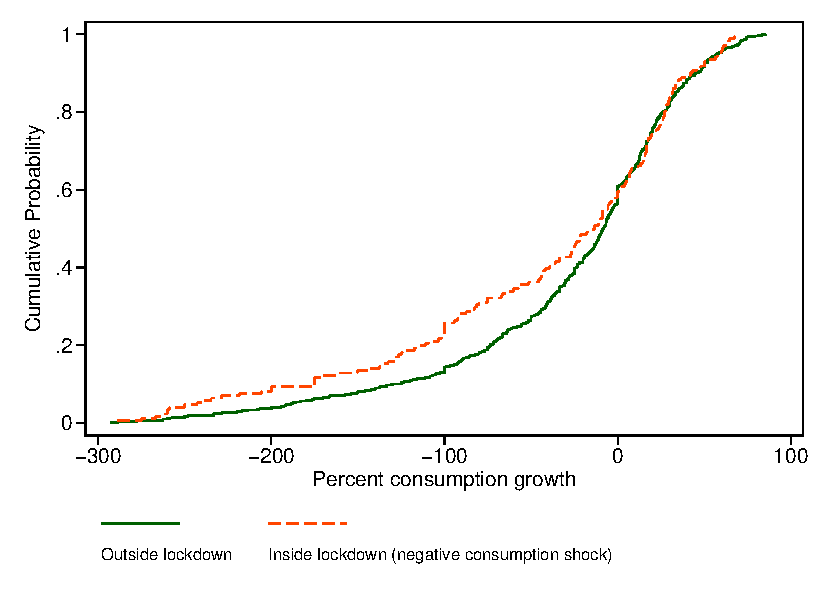
\includegraphics[scale=1.2]{../3-replication-package/Output/Figures/figure_a10}}{\large\par}
\par\end{centering}
{\small Note: Figure plots the distribution (CDF) of consumption growth
per week at endline for the different subsamples (lockdown areas vs
non-lockdown areas). Observations are at the individual level. Median
(mean) percent consumption growth is -13\% (-45\%) for individuals
in lockdown areas and -8\% (-27\%) for those in non-lockdown areas.
From a Kolmogorov--Smirnov (KS) test for the equality of distributions,
}{\small\textit{p}}{\small -value equals 0.020 (for equality test,
we trimmed the individual consumption growth outcome at the 5\% level).
Equality tests reject the null that the distributional pairs are equal.}{\small\par}
\end{figure}
}{\large\par}
\par\end{center}

\newpage{}

\subsection{Definition of Relevant Select Variables -- Questions}

\begin{doublespace}
\noindent{\large\textbf{Communication constraints (un)mitigation: }}{\large\par}
\end{doublespace}

\noindent{\large Consider the last 7 days: }{\large\par}
\begin{enumerate}
\item {\large Unable to call in past 7days 0-1: }{\large\texttt{Were you
confronted with the need to call others (i.e., family, friends or
work) but unable to call because you/ household lacked enough communication
resources to cover costs? 0=No, 1=Yes}}{\large\par}
\item {\large Borrow airtime 0-1: }{\large\texttt{Have borrowed airtime due
to unexpected circumstances to make calls? 0=No, 1=Yes }}{\large\par}
\item {\large Seek digital loan 0-1: }{\large\texttt{Have taken a digital
loan due to unexpected circumstances to make calls? 0=No, 1=Yes}}{\large\par}
\item {\large Unable to call due to COVID19 0-1: }{\large\texttt{Are you
sometimes unable to see or communicate with your family and friends
due to COVID19, its lockdown restrictions and other personal avoidance
steps you have taken? 0=No, 1=Yes }}{\large\par}
\end{enumerate}
\begin{doublespace}
\noindent{\large\textbf{Gender and Domestic violence relations: }}{\large\par}
\end{doublespace}

\noindent{\large Consider last 7 days: Please indicate how often you
act to the following:}\textbf{ }

\noindent\textbf{USE CODES:}

\noindent{\large\texttt{1=Never (less than 1 time in 7 days), 2=Sometime
(1-2 times in 7 days), 3=Often (3-4 times in 7 days), 4=Very often
(5-7 times in 7 days), 5=No Answer (if you want/feel uncomfortable
to say)}}{\large\par}
\begin{enumerate}
\item {\large Threatened Partner 1-4:}{\large\texttt{ How often do you threaten
to hurt your partner or someone close to your partner? }}{\large\par}
\item {\large Hit Partner 1-4:}{\large\texttt{ How often do you hit or throw
something at your partner? }}{\large\par}
\end{enumerate}
\begin{doublespace}
\noindent{\large\textbf{Mental Health (K10):}}{\large\par}
\end{doublespace}

\noindent{\large Consider last 7 days: Please indicate how often you
feel about the following: }{\large\par}

\noindent\textbf{USE CODES:}

\noindent{\large\texttt{1=None of the time (less than 1 time in 7
days), 2=A little of the time (1-2 times in 7 days), 3=Some of the
time (3-4 times in 7 days) 4=Most of the time (5-6 times in 7 days),
5=All of the time (7 times in 7 days) }}{\large\par}
\begin{enumerate}
\item {\large\texttt{About how often did you feel tired out for no good
reason? }}{\large\par}
\item {\large\texttt{About how often did you feel nervous? }}{\large\par}
\item {\large\texttt{About how often did you feel nervous that nothing could
calm you down? }}{\large\par}
\item {\large\texttt{About how often did you feel hopeless? }}{\large\par}
\item {\large\texttt{About how often did you feel restless or fidgety? }}{\large\par}
\item {\large\texttt{About how often did you feel so restless you could
not sit still? }}{\large\par}
\item {\large\texttt{About how often did you feel depressed? }}{\large\par}
\item {\large\texttt{About how often did you feel that everything was an
effort? }}{\large\par}
\item {\large\texttt{About how often did you feel so sad that nothing could
cheer you up? }}{\large\par}
\item {\large\texttt{About how often did you feel worthless?}}{\large\par}
\end{enumerate}
\noindent{\large\textbf{Consumption Expenditures (weekly):}}{\large\par}
\begin{enumerate}
\item {\large\texttt{What is the total value (in GHS) of all food and beverage
items your household (i) purchased and consumed, (ii) consumed from
your own stock or production, or (iii) received as a gift and consumed
over the last 7 days? NOTE: Please only include food and beverage
items consumed in the 7 days ...GHS }}{\large\par}
\item {\large\texttt{What is the total value (in GHS) of all food and beverage
items you or any member of your household purchased and consumed from
outside the house over the last 7 days? NOTE: This includes items
purchased outside the house in restaurants, cafeterias, canteens/kiosks,
as well as products such as spirits, tobacco, stimulants, etc. ...GHS}}{\large\par}
\item {\large\texttt{What is the total value (in GHS) of house rents, house
repair costs and utilities that were paid for, purchased, or acquired
from other sources (ie gifts and in-kind) by your household over the
last 7 days? NOTE: Utilities include sewerage, electricity, water,
gas, cooking fuels, house servants, etc. ...GHS }}{\large\par}
\item {\large\texttt{What is the total value (in GHS) of products and services
for personal use and care, that were paid for, purchased, or acquired
from other sources (ie gifts and in-kind) over the last 7 days by
your household? NOTE: Personal care products and services include
barber services, electrical appliances for personal care, oils, soaps,
etc. Personal use products and services include jewelry, accessories
(watches, clocks, clothing, etc.), cultural services, mobile airtime
services, financial service fees, transportation costs. ...GHS }}{\large\par}
\item {\large\texttt{What is the total value (in GHS) of education expenses
(i.e., all tuition or fees including all educational scholarships)
over the last 7 days by your household? ...GHS }}{\large\par}
\item {\large\texttt{What is the total value (in GHS) of consultation or
treatment services, and pharmaceutical or therapeutic products purchased
last 7 days by your household? ...GHS }}{\large\par}
\item {\large\texttt{What is the total value (in GHS) of durable products
such as furniture, electronics and other household appliances, purchased
over the last 7 days by your household? NOTE: This includes furniture,
household appliances (large and small), repair of household appliances,
miscellaneous accessories such as TVs, laptops, cars, mobile phones,
bicycles, torches, batteries, solar lamps, etc. ...GHS }}{\large\par}
\item {\large\texttt{Total expenditure: add 1 to 8 ...GHS}}
%
\end{enumerate}
\newpage{}
\begin{doublespace}

\subsection{Marginal Value of Public Funds (MVPF)}
\end{doublespace}

\begin{doublespace}
\noindent{\large We use our causal estimates to compute the MVPF (Hendren
and Sprung-Keyser 2020) for a policy that provides communication credit
to low-income adults for two months. The MVPF is a ratio of society’s
willingness to pay (private benefit) for this policy to the net cost
of the policy to the government (here, an ``imagined'' funder). }{\large\par}
\end{doublespace}
\begin{doublespace}

\subsubsection{{\large Society’s Willingness to Pay (MVPF numerator)}}
\end{doublespace}

\begin{doublespace}
\noindent{\large We estimate this to include two main components. }{\large\par}
\end{doublespace}

\begin{doublespace}
{\large First, is the averted (otherwise) social cost of mental health
burden, $\xi$. Mental health disorders account for 13\% of the overall
global disease burden (Collins et al. {[}2011{]}), which is likely
higher in low-income countries (\href{https://www.journals.uchicago.edu/doi/full/10.1086/701606?mobileUi=0}{Adhvaryu et al. [2019]});
we assume 13\%. Health expenditure per capita in Ghana is US\$78 (\href{https://data.worldbank.org/indicator/SH.XPD.CHEX.PC.CD?locations=GH}{World Bank [2018]}).
With a treatment effect of -10\% reduced mental destress rate (or
-25\% for severe mental distress; we assume -10\%), we conservatively
estimate the averted social cost of mental health burden to be 0.10x0.13xUS\$78=+US\$1.014.
This $\xi$ estimate is very conservative: \href{https://pubmed.ncbi.nlm.nih.gov/24526584/}{Addo et al. [2013]}
estimate that the average monthly household cost of mental healthcare
in Ghana is US\$60.24 (i.e., 2xUS\$60.24=US\$120.48 for two months),
so with a treatment effect of -10\% reduced mental destress rate and
a national average household size of 4.5 people per household, this
will imply 0.1xUS\$120.48/4.5=+US\$2.68 averted social cost, which
is 2.6 times larger. Second, is the individual beneficiary's willingness
to pay for not visiting the hospital or not getting mentally unwell,
$\eta$. This includes three sub-components: (i) out-of-pocket health
bill $\eta_{1}$ (0.10x0.13xUS\$63=+US\$0.82; out-of-pocket health
expense is US\$63 {[}\href{https://data.worldbank.org/indicator/SH.XPD.CHEX.PC.CD?locations=GH}{World Bank 2018}{]});
(ii) travel cost to health centers $\eta_{2}$ (assumed to be 20\%
of the estimated out-of-pocket health bill = 0.2xUS\$0.82=+US\$0.203;
\href{https://pubmed.ncbi.nlm.nih.gov/24526584/}{Addo et al. [2013]}
suggest using 74\% for such indirect costs but we assume 20\%); and
(iii) lost income from missed work $\eta_{3}$ (assumed to be only
5\% of the average earnings of non-farm enterprises = 0.05xUS\$231=+US\$11.55
for two months; most individuals in our sample {[}around 80\%{]} operate
informal non-farm enterprises and the total average annual earnings
of non-farm enterprises is US\$1,385 in 2021 US\$ {[}\href{https://www.statsghana.gov.gh/gssmain/fileUpload/pressrelease/GLSS7\%20MAIN\%20REPORT_FINAL.pdf}{Ghana Statistical Service, GLSS 7 Table 9.6]};
the treatment effects were all concentrated on individuals operating
informal enterprises, see Table \ref{tab:wellbeingXinformal_pooled_meta}).}{\large\footnote{{\large Informal non-farm business income may either be consumed in
the household (where we find no impacts) or invested (where our impacts
are concentrated given that our treatment effects were all concentrated
on individuals operating informal enterprises).}}}{\large\par}

{\large Combining all the components, the MVPF's numerator = $\xi$+$\sum_{i=1}^{3}\eta_{i}$=US\$13.590
for the average treated individual.}{\large\footnote{{\large We drop the direct value of the communication subsidy to beneficiaries
(+US\$7.0) to avoid double counting. In standard maximization models,
the willingness to pay would have just been the size of the subsidy
}{\large\textit{if}}{\large{} people are fully optimizing. Here, it
is reasonable to assume that people are not fully optimizing (see
e.g., our evidence that the installment program has larger and more
sustainable effects compared to the lumpsum, with the exception of
consumption, which may reflect either time inconsistency or social
pressure problems from receiving one-time large transfers). Given
this potential mis-optimization (the envelope theorem does not easily
apply and so the benefits the subsidy delivers to people are not already
captured by the subsidy), the willingness to pay includes the benefits
on mental health and its associated cost reductions ($\xi$ and $\eta$).}}}{\large .}{\large\par}
\end{doublespace}
\begin{doublespace}

\subsubsection{{\large Net Cost to the \textquotedblleft imagined\textquotedblright{}
Funder / Government (MVPF denominator)}}
\end{doublespace}

\begin{doublespace}
\noindent{\large We estimate this to include two main components. }{\large\par}
\end{doublespace}

\begin{doublespace}
{\large First, is the cost of providing communication transfer for
two months, $G$ (+US\$7.0). Second, is the missed communication services
tax (CST) revenue if individuals do not communicate or stay connected,
$\mu$. In Ghana, the CST is used to finance the National Youth Employment
Programme (NYEP) ($\geq$20\% of the CST) and support other national
development activities. Using the prevailing 5\% CST rate (\href{https://gra.gov.gh/news/amendments-to-the-communications-service-tax-act-2008-act-754/}{Ghana Revenue Authority [2020]}),
we estimate that the government loses 0.05xUS\$7.0= -US\$0.35. In
computing the net cost to the government of this policy, it is important
to note that (i) communication is a network good so the ultimate economic
incidence of these communication transfers extends to other individuals:
others might benefit from receiving mobile phone calls from the treated
individual (positive externalities) but this might also create congestion
hassle or traffic on the communication network (negative externalities).
We assume (i) and (ii) to be equal. If the positive externalities
dominate, as we would expect (see \href{https://academic.oup.com/restud/article/86/3/1033/5061115?guestAccessKey=8628aed3-426d-4fc6-af39-bd5561c493a3}{Björkegren [2019]}
for an example in Rwanda), then the total cost of this policy is over-estimated
in this dimension. Further, we conservatively did not factor in the
reduced fiscal cost from less hospital visits generally due to the
reduced likelihood of mental health disorders. }{\large\par}

{\large Lastly, combining all the components, the MVPF's denominator
= $G$+$\mu$=US\$6.65 for the average treated individual. }{\large\par}
\end{doublespace}
\begin{doublespace}

\subsubsection{{\large MVPF Estimate}}
\end{doublespace}

\begin{doublespace}
\noindent{\large Taking the ratio, we estimate a conservative MVPF
of providing communication credit to be $\frac{13.590}{6.650}=2.044$.
Notice that in determining the MVPF, we intentionally bias the estimates
to understate the benefits and overstate the costs. With a current
total population of about 31,732,129 in Ghana, an adult population
of 18,073,230 (57\% of the total population), and the poverty rate
of our study's sample of adults being 22\%, the policy's total benefit
will be US\$54,035,343 (=0.22x18,073,230xUS\$13.590) against a total
cost of US\$26,441,135 (=0.22x18,073,230xUS\$6.650).}{\large\par}
\end{doublespace}
\selectlanguage{american}%

\end{document}
